\subsection{Компьютерные сети}
	
	\subsubsection{Аннотация}

        Курс <<Компьютерные сети>> получил смешанные отзывы. 
        
        Лекции Климанова М.М. получили высокие оценки за качество изложения материала, но система оценивания и организация учебного процесса вызвали множество нареканий. 
        
        Лабораторные работы также нуждаются в серьезной доработке, особенно в части взаимодействия преподавателей со студентами.

        Руководствуясь результатами опроса, Совет студентов и аспирантов ФРКТ выдвигает следующие идеи по улучшению данного курса:
        \begin{enumerate}
            \item пересмотреть критерии оценивания, чтобы студенты могли рассчитывать свою оценку в течение семестра;
            \item увеличить время на выполнение контрольных работ;
            \item добавить больше практических занятий (например, вместо лаборатории инфокоммуникационных технологий сделать семинар), где студенты могли бы решать задачи, аналогичные тем, что даются на контрольных;
            \item вместо устаревших тем, например STP, рассказывать более актуальные темы.
        \end{enumerate}	

	\subsubsection{Общий отзыв студентов о курсе}

		\begin{figure}[H]
			\centering
			\begin{subfigure}[b]{0.45\textwidth}
				\centering
				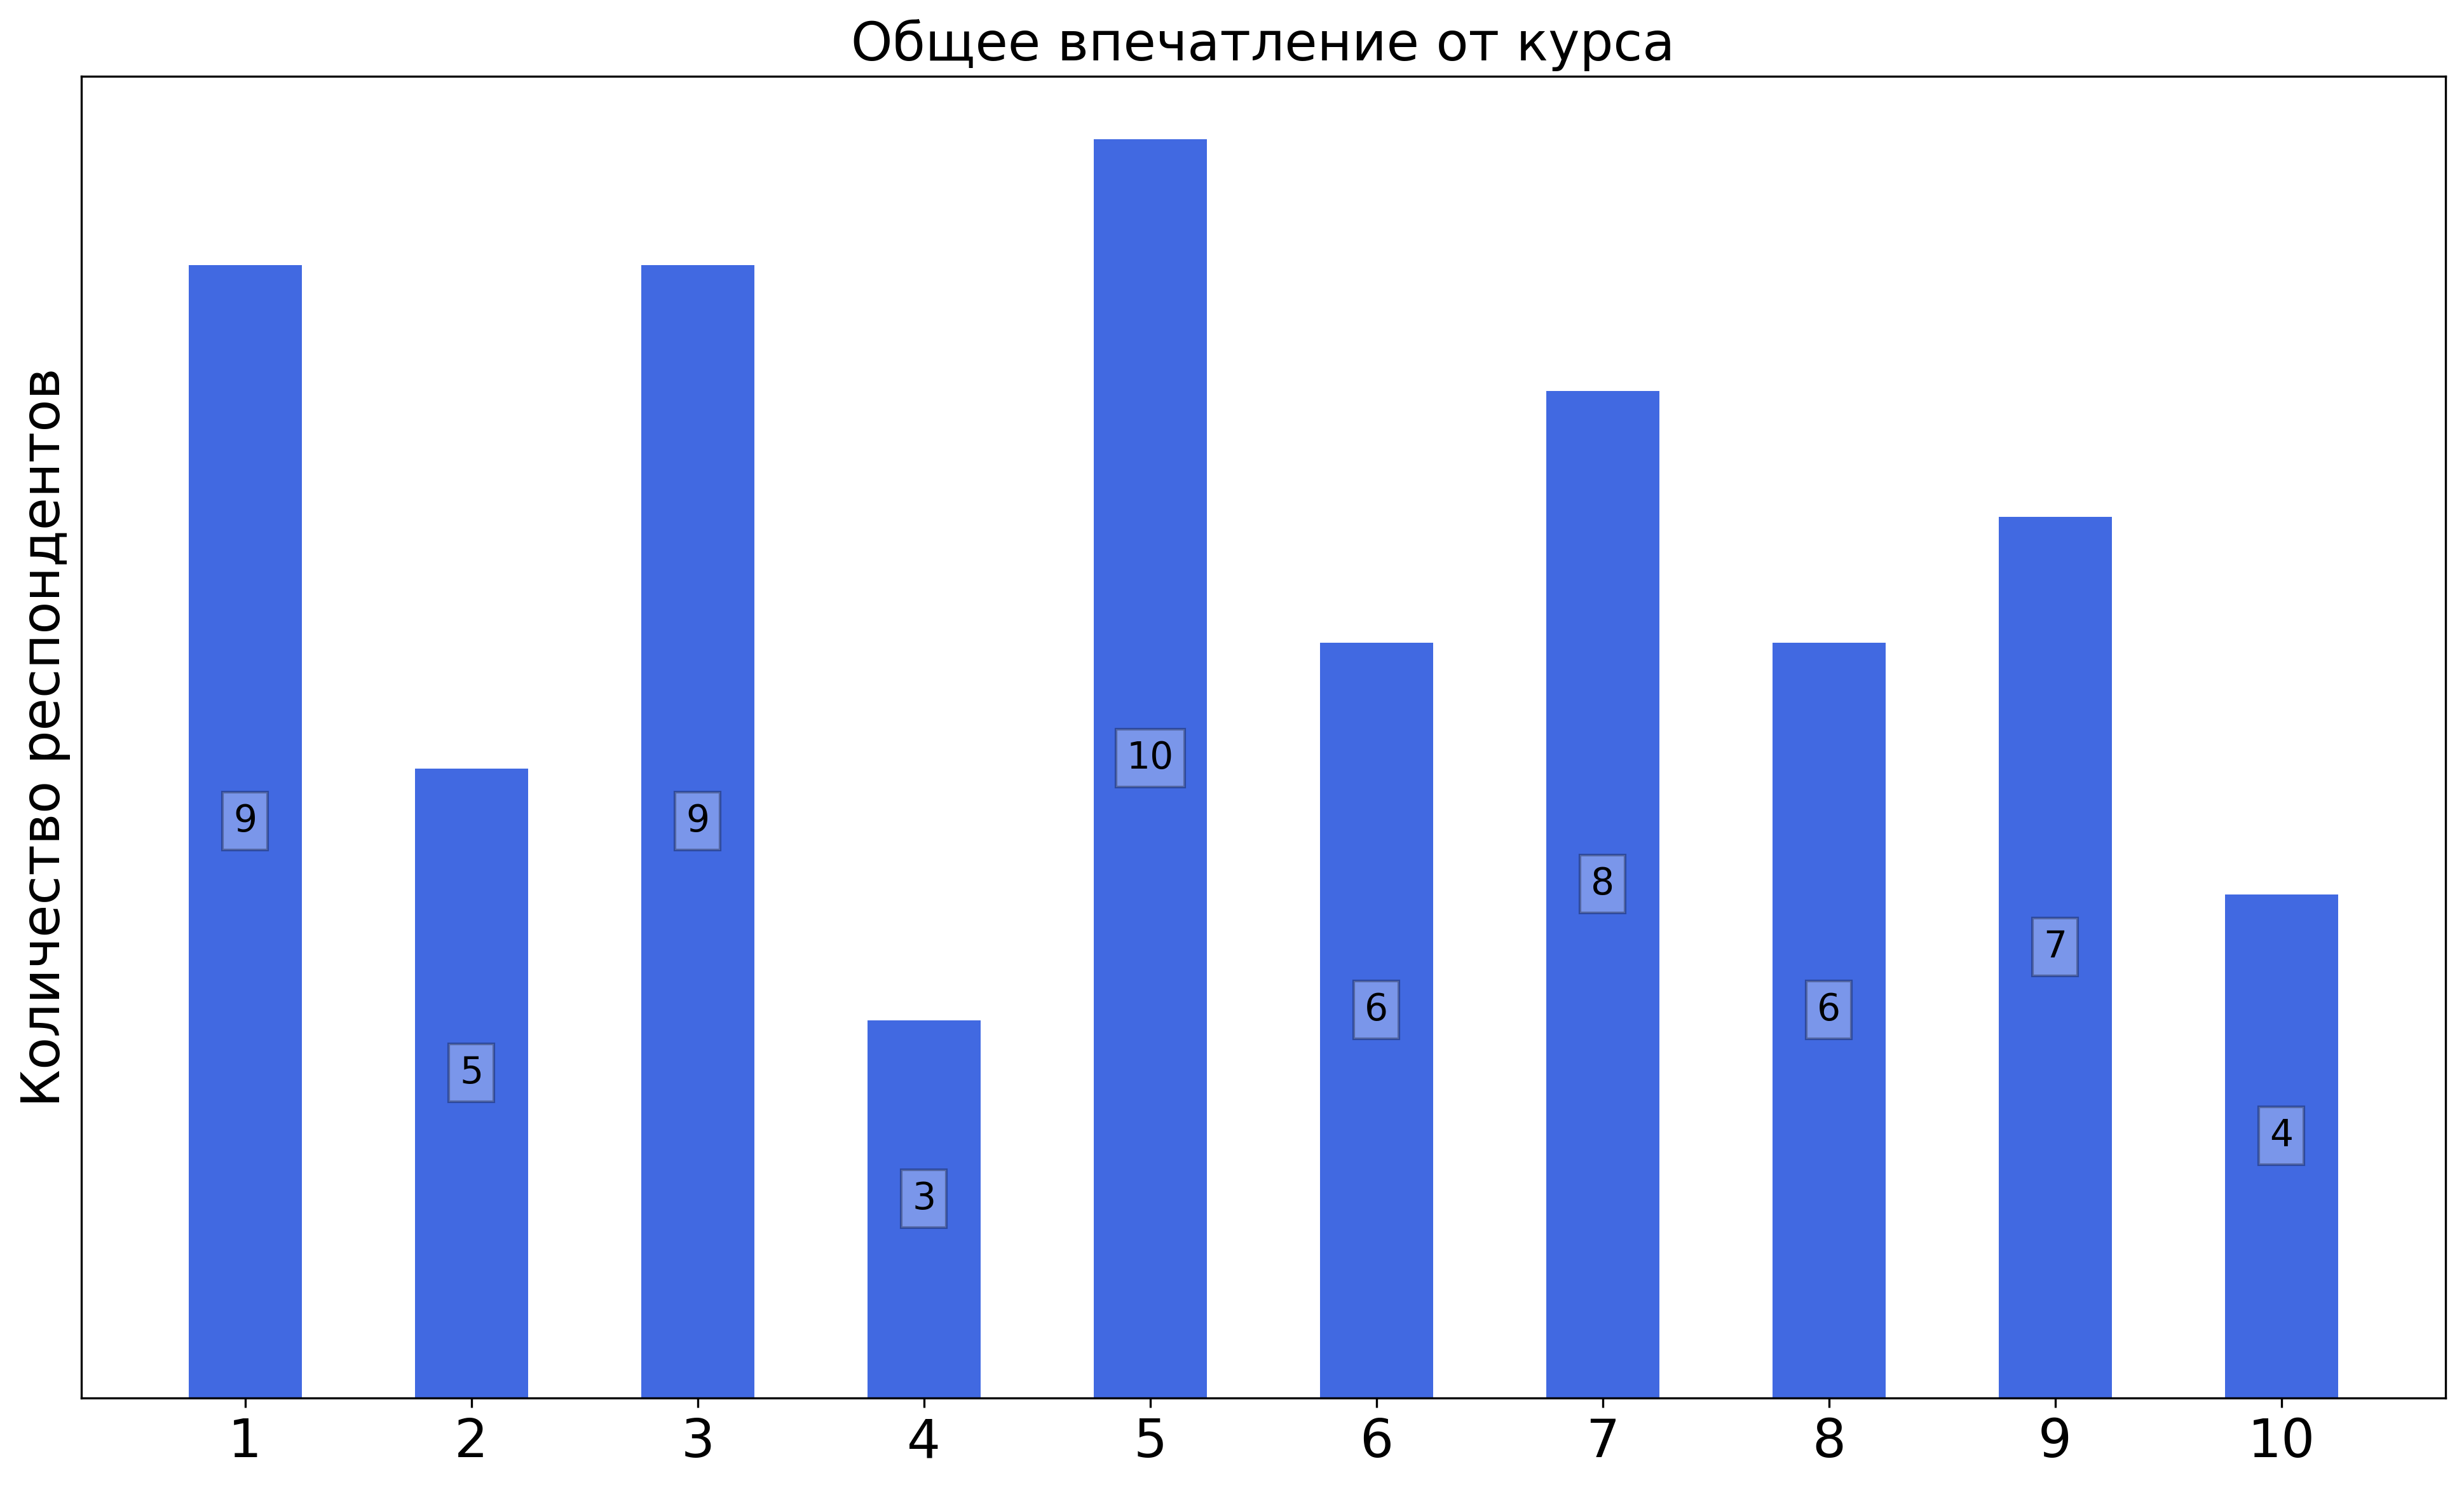
\includegraphics[width=\textwidth]{images/3 course/Компьютерные сети/general-0.png}
			\end{subfigure}
		\end{figure}

	\subsubsection{Материалы, использумые респондентами при изучении курса}

		\begin{figure}[H]
			\centering
			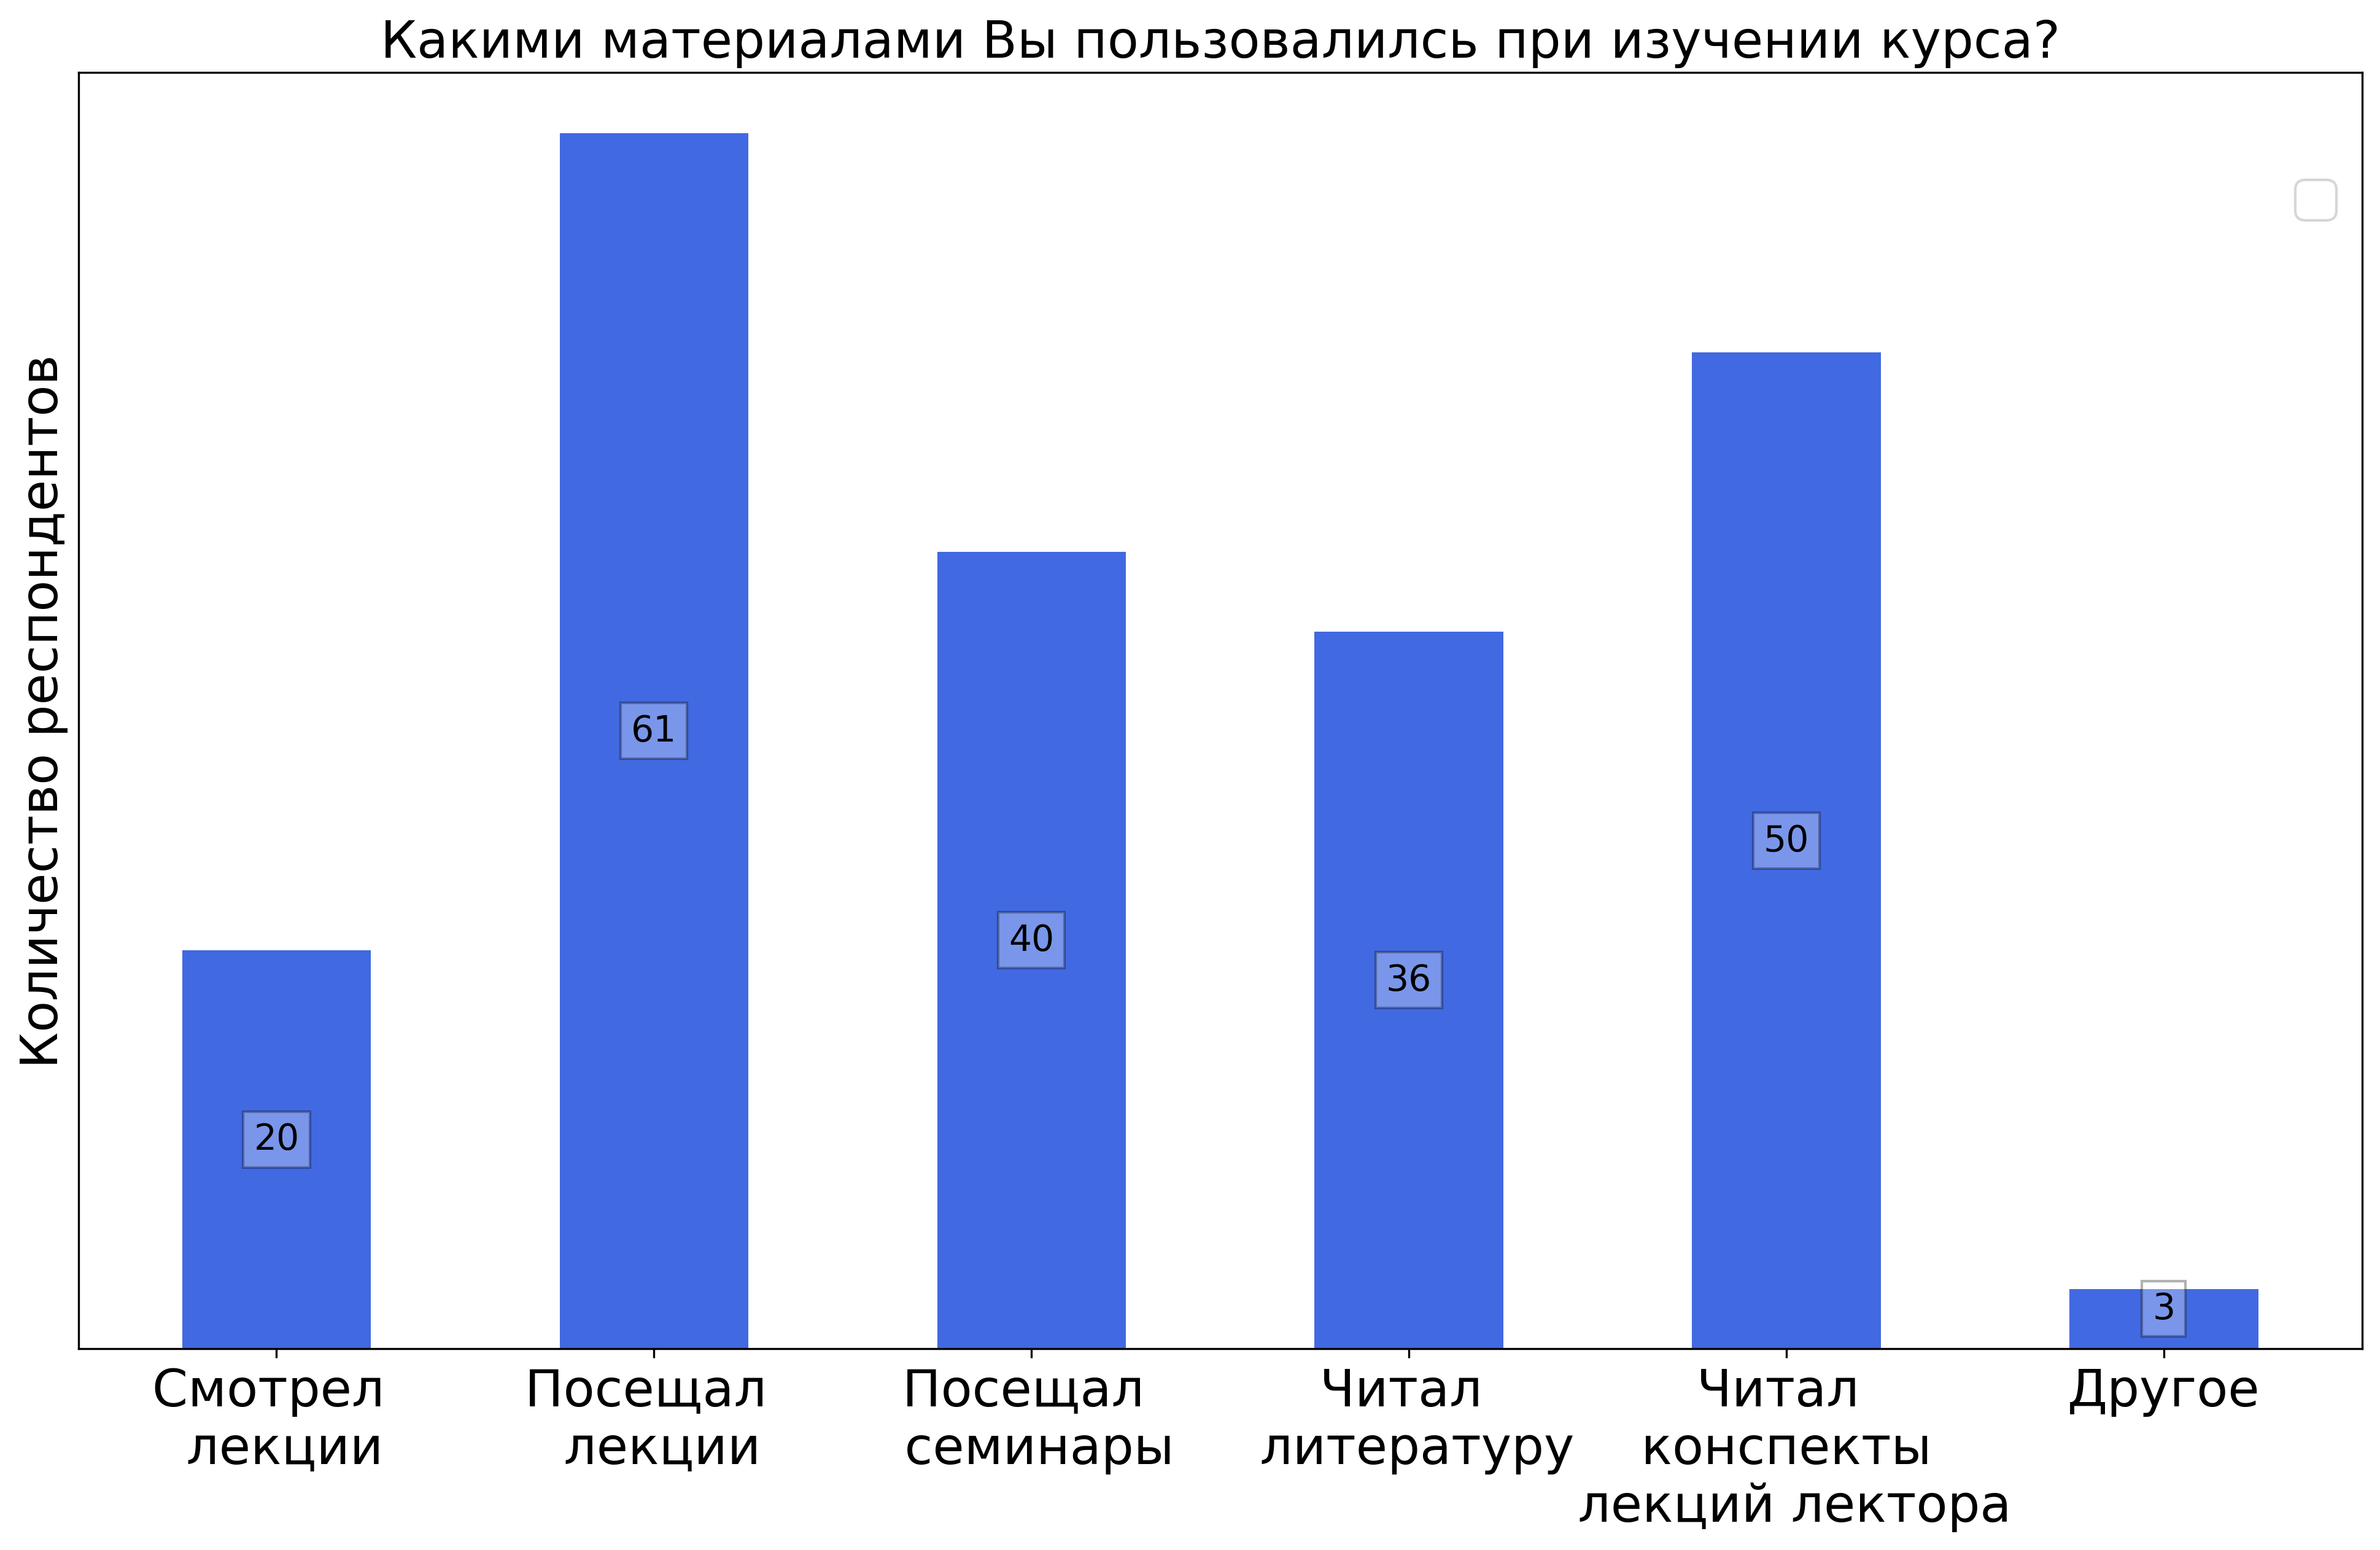
\includegraphics[width = 0.45\textwidth]{images/3 course/Компьютерные сети/materials.png}
		\end{figure}

		\textit{В качестве других источников информации студенты указали:} 
		\begin{itemize}
			\item методички к лабораторным работам.
		\end{itemize}

	\subsubsection{Отзыв студентов о лекциях. Лектор: Климанов М.М.}

		\begin{figure}[H]
			\centering
            \begin{subfigure}[b]{0.45\textwidth}
				\centering
				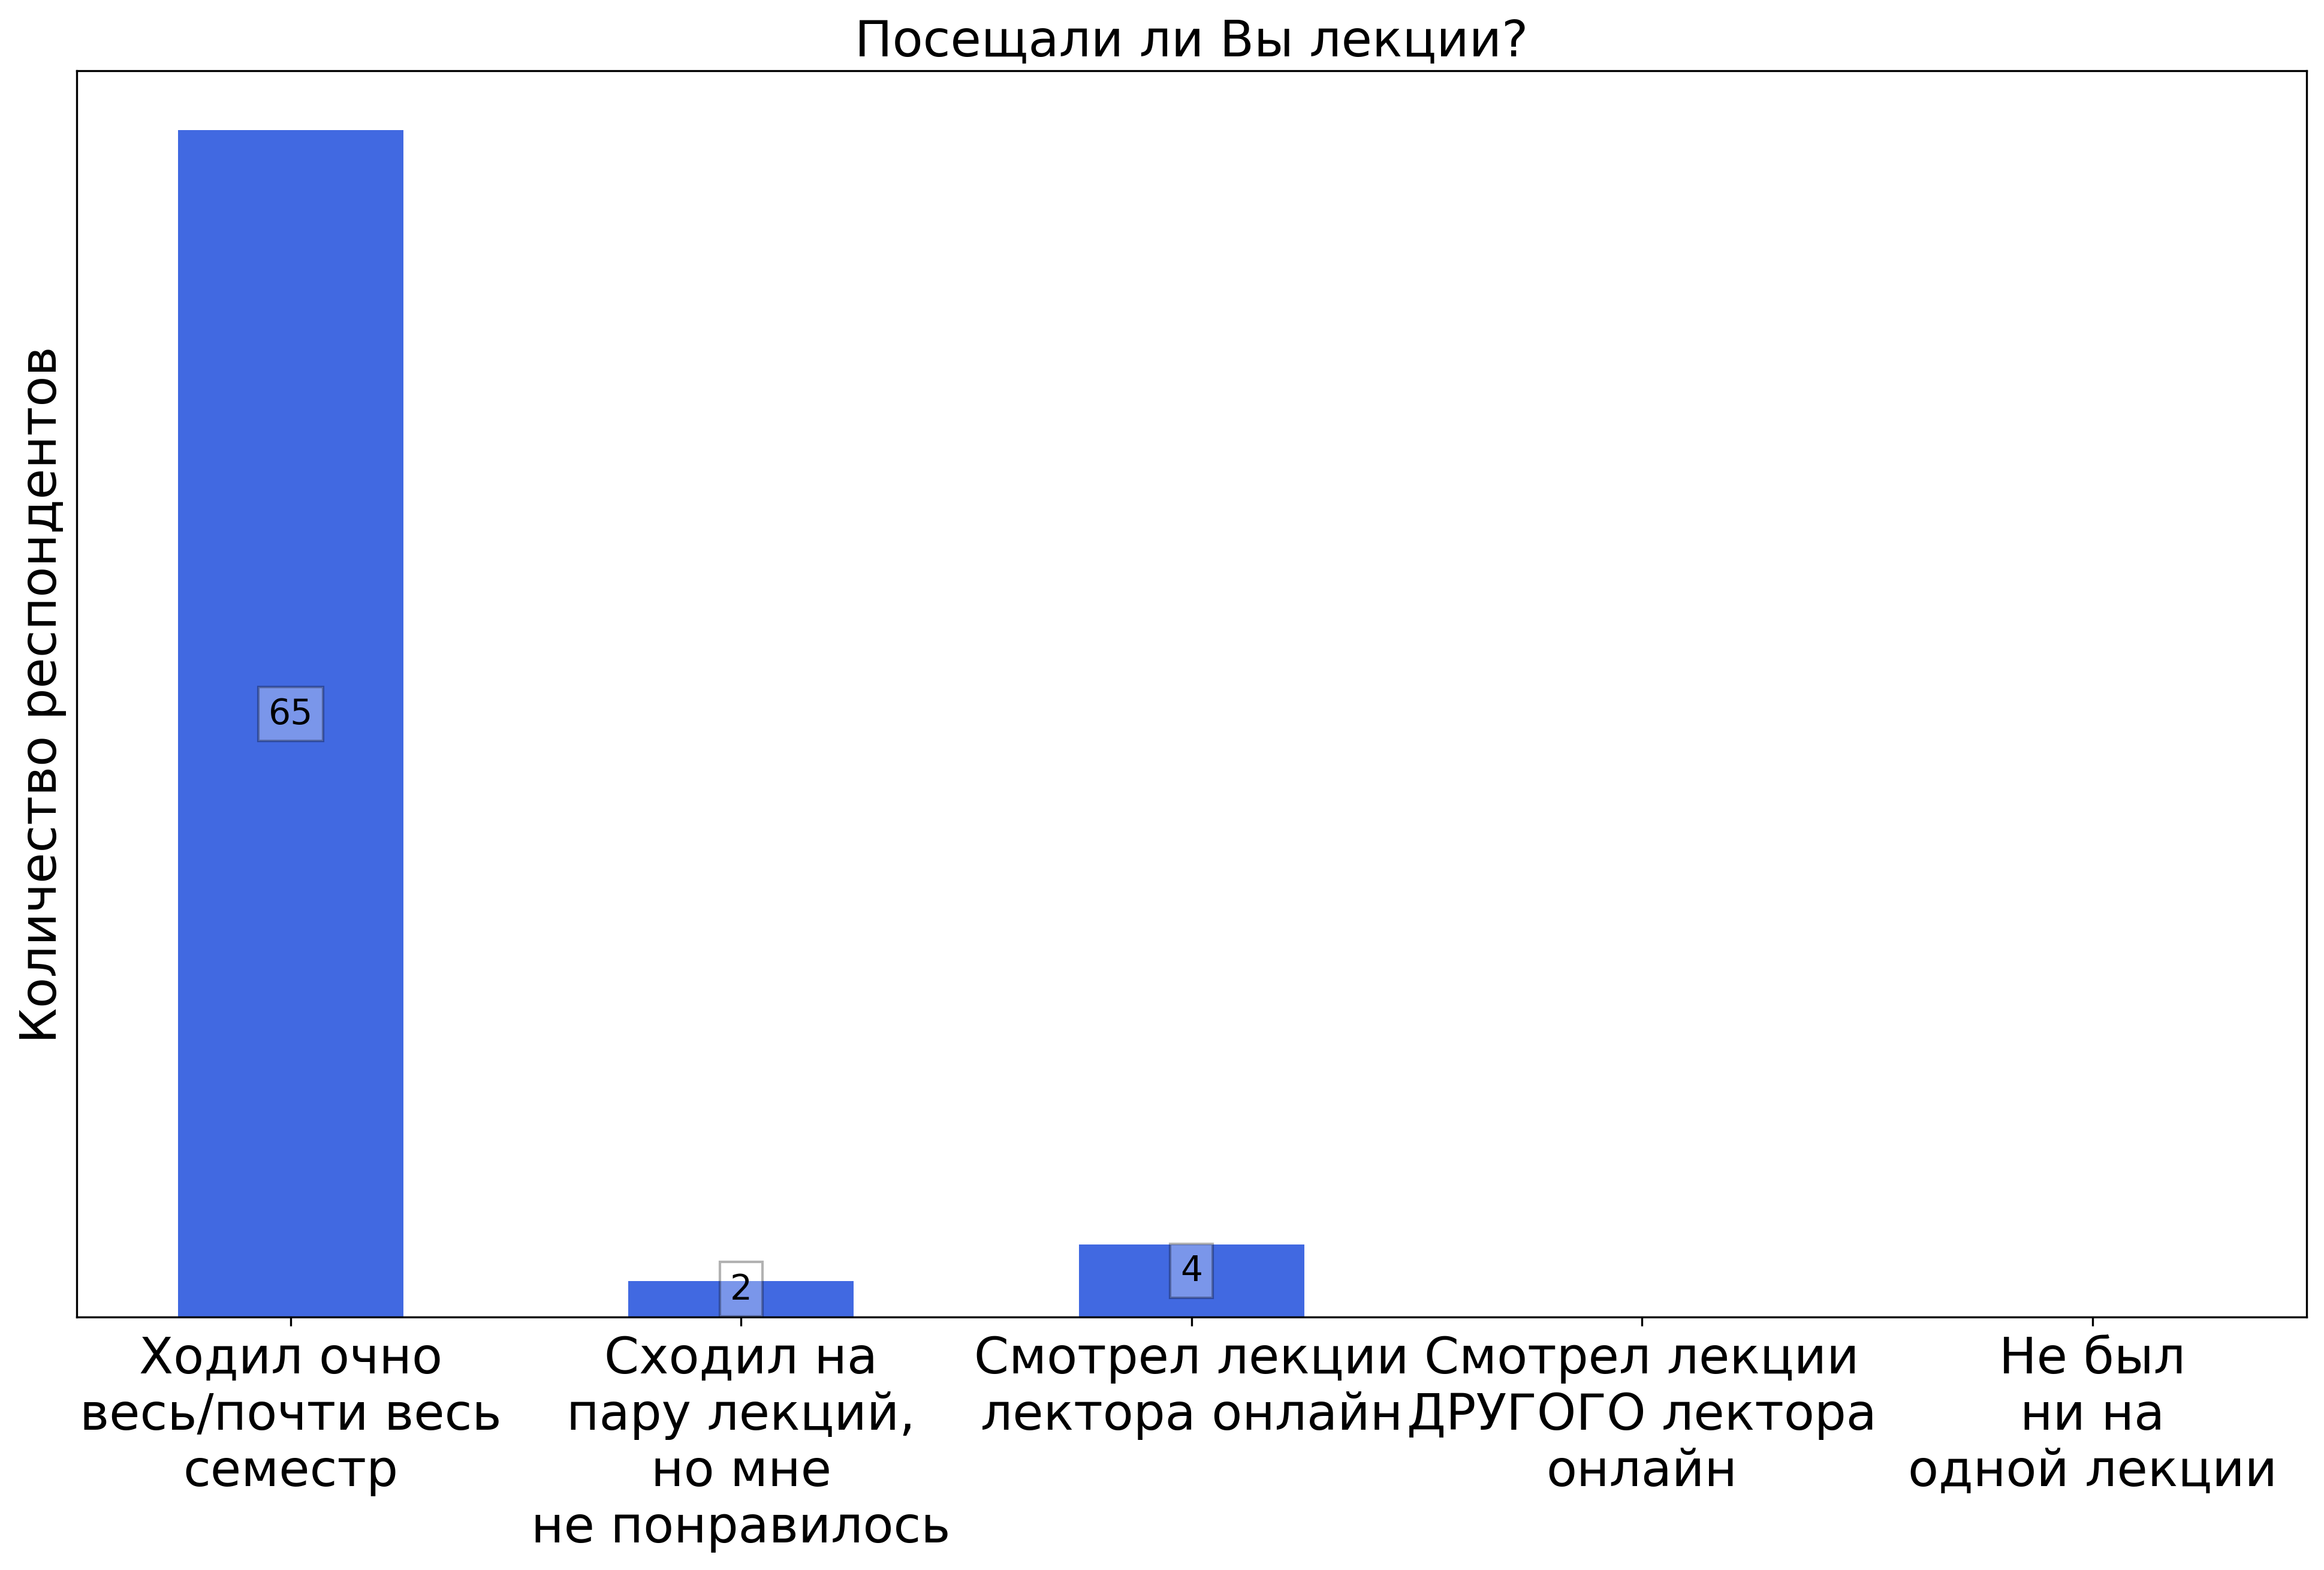
\includegraphics[width=\textwidth]{images/3 course/Компьютерные сети/lecturer-questions-Климанов М.М.-0.png}
			\end{subfigure}
			\begin{subfigure}[b]{0.45\textwidth}
				\centering
				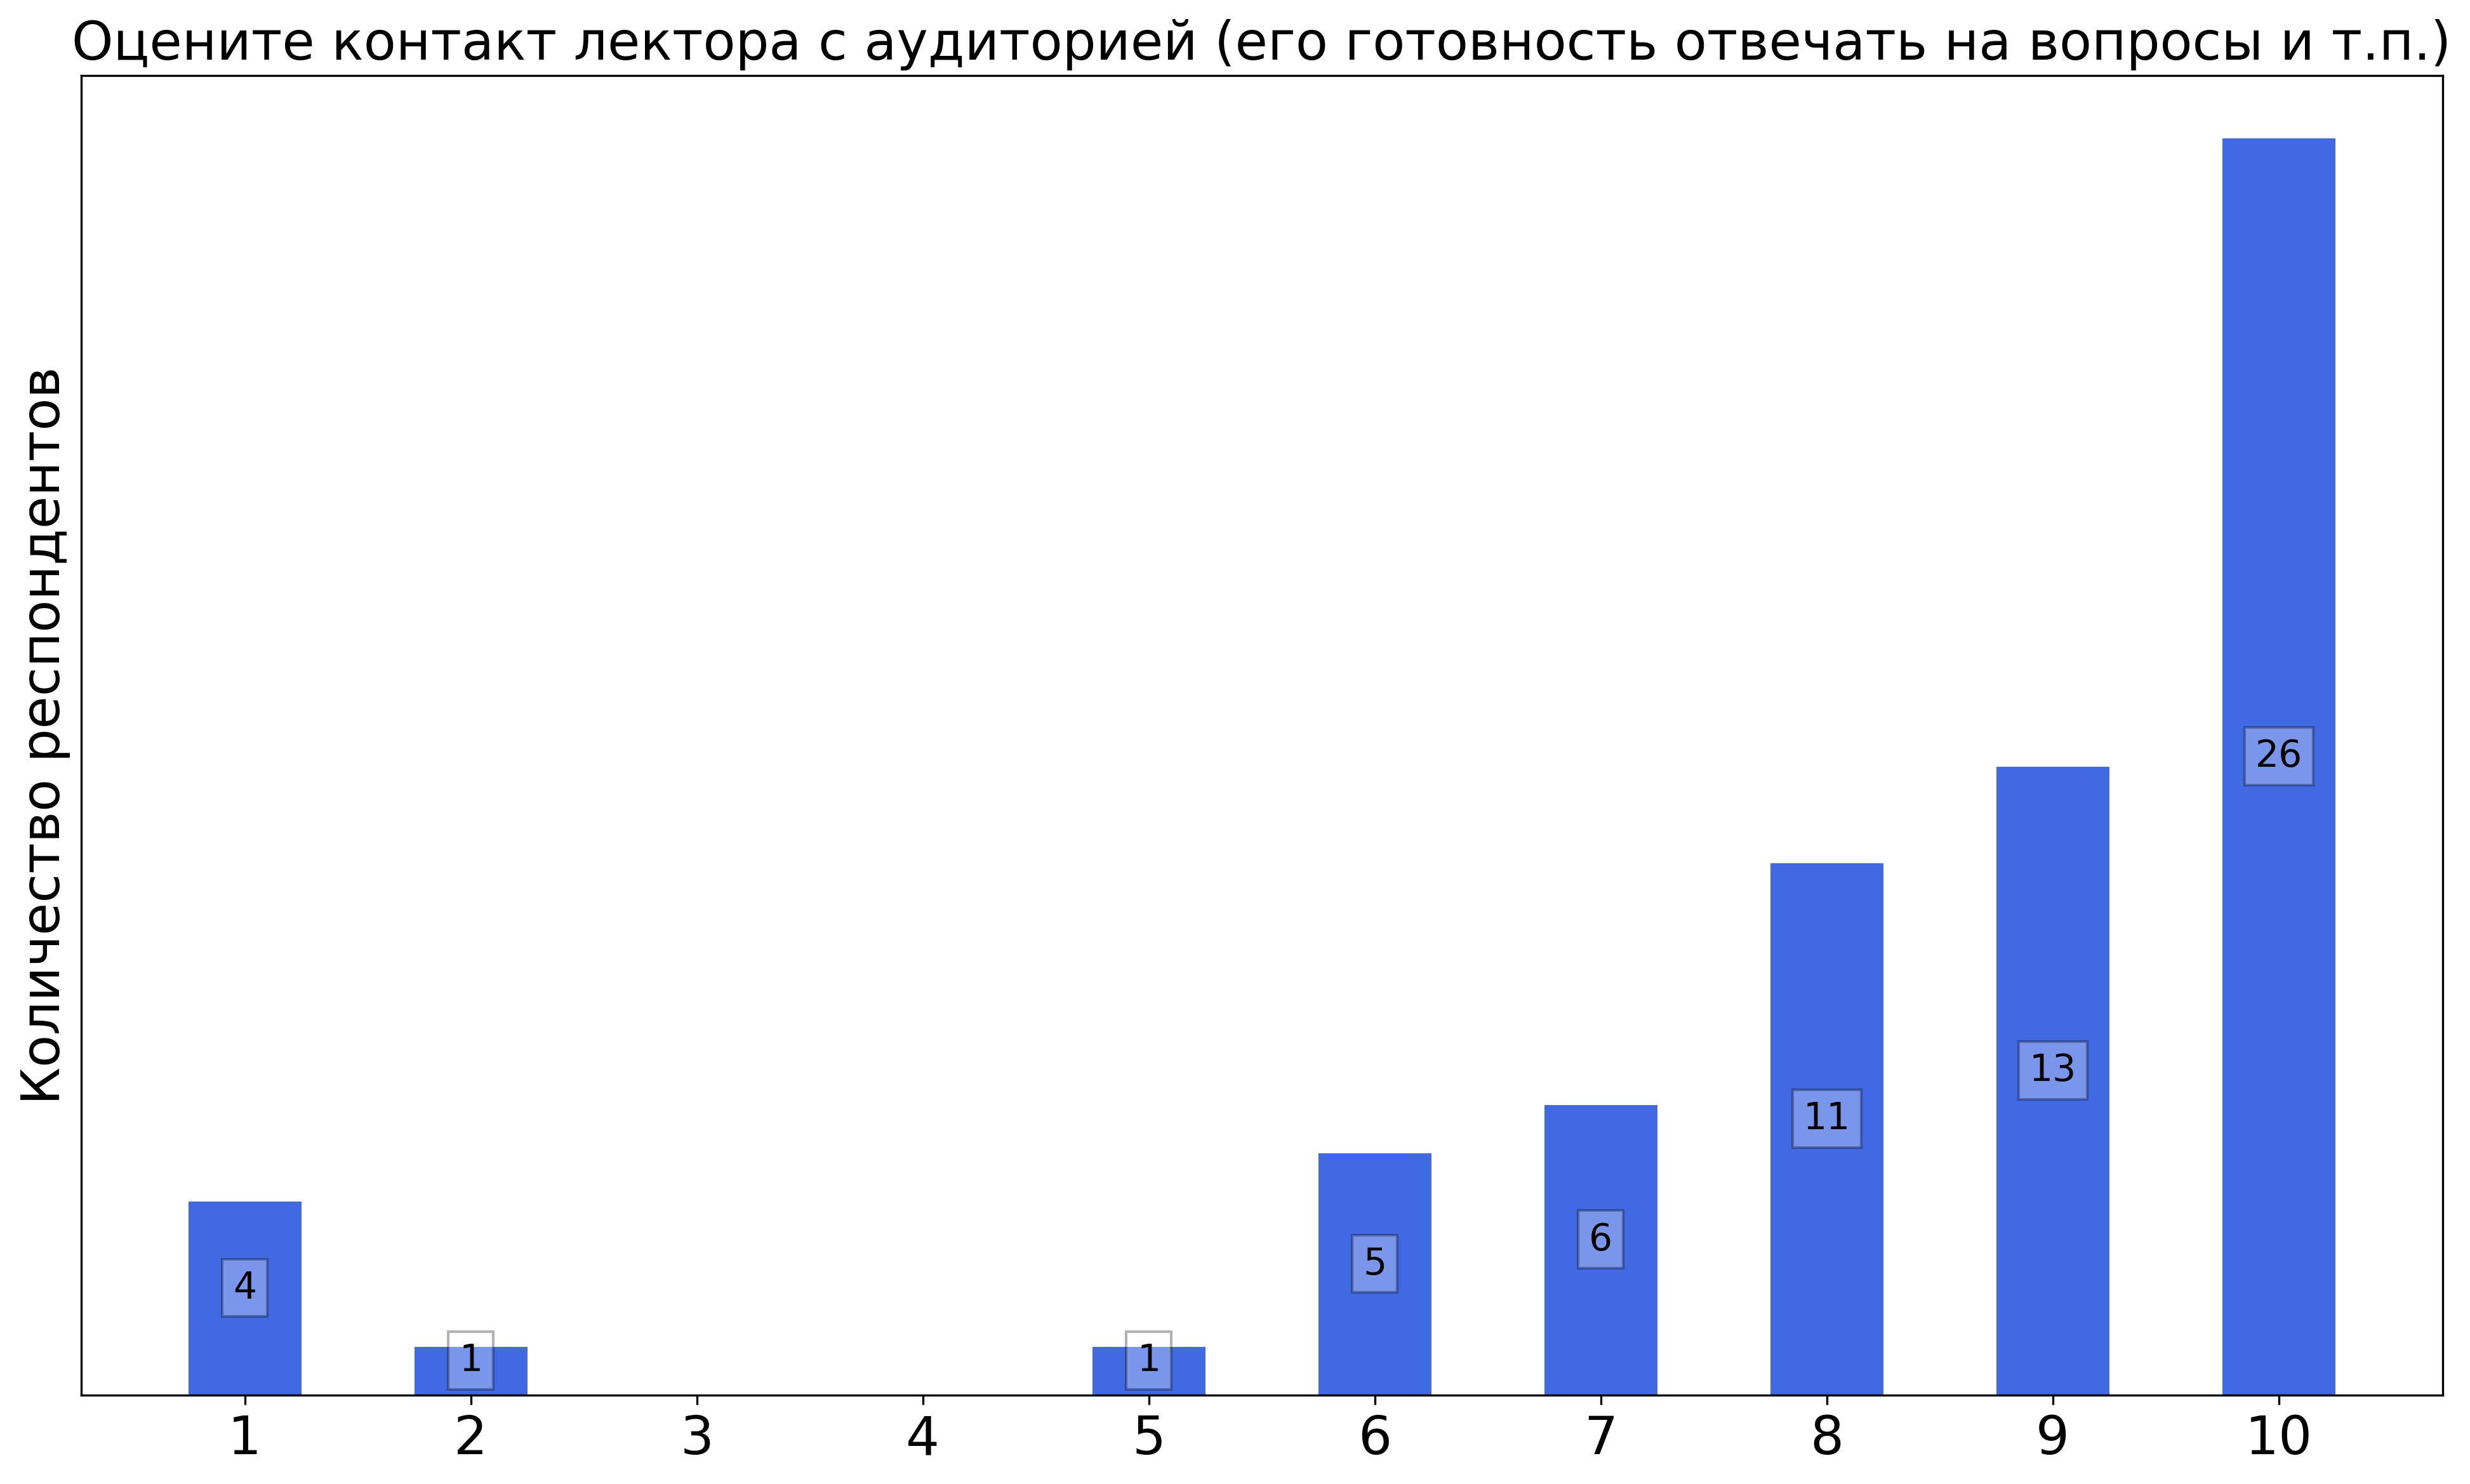
\includegraphics[width=\textwidth]{images/3 course/Компьютерные сети/lecturer-marks-Климанов М.М.-0.png}
			\end{subfigure}
			\begin{subfigure}[b]{0.45\textwidth}
				\centering
				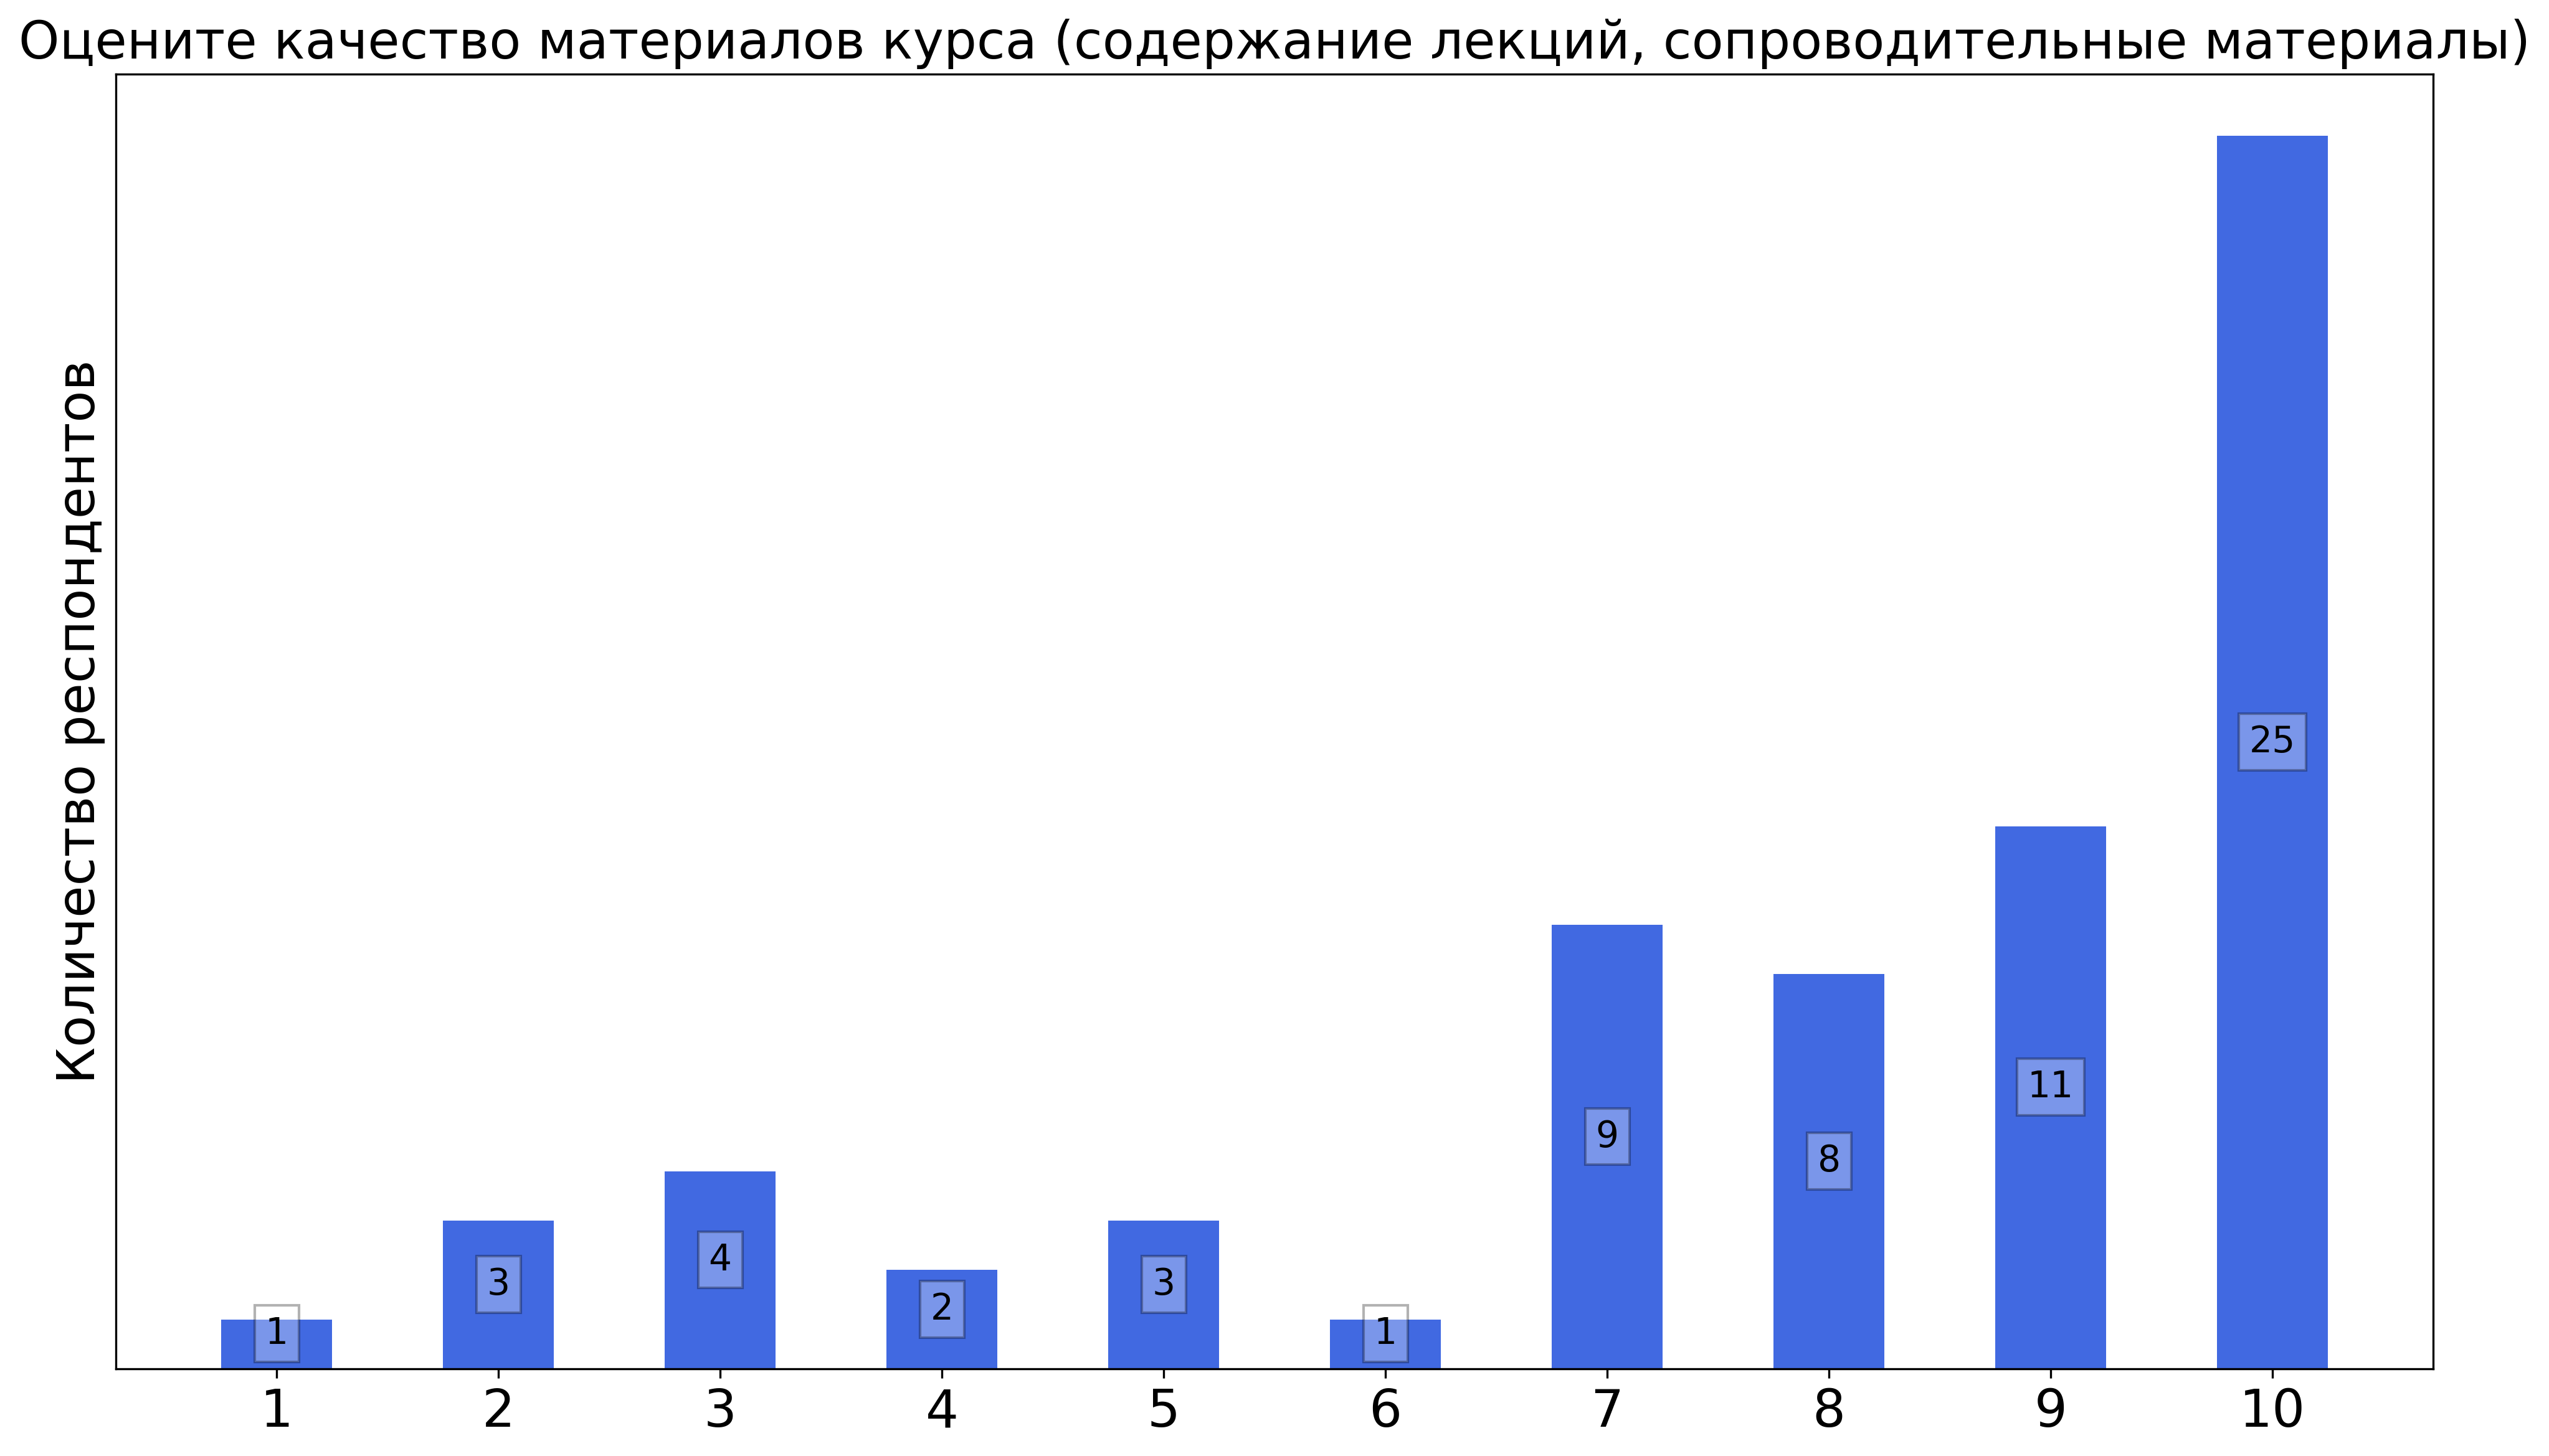
\includegraphics[width=\textwidth]{images/3 course/Компьютерные сети/lecturer-marks-Климанов М.М.-1.png}
			\end{subfigure}
			\begin{subfigure}[b]{0.45\textwidth}
				\centering
				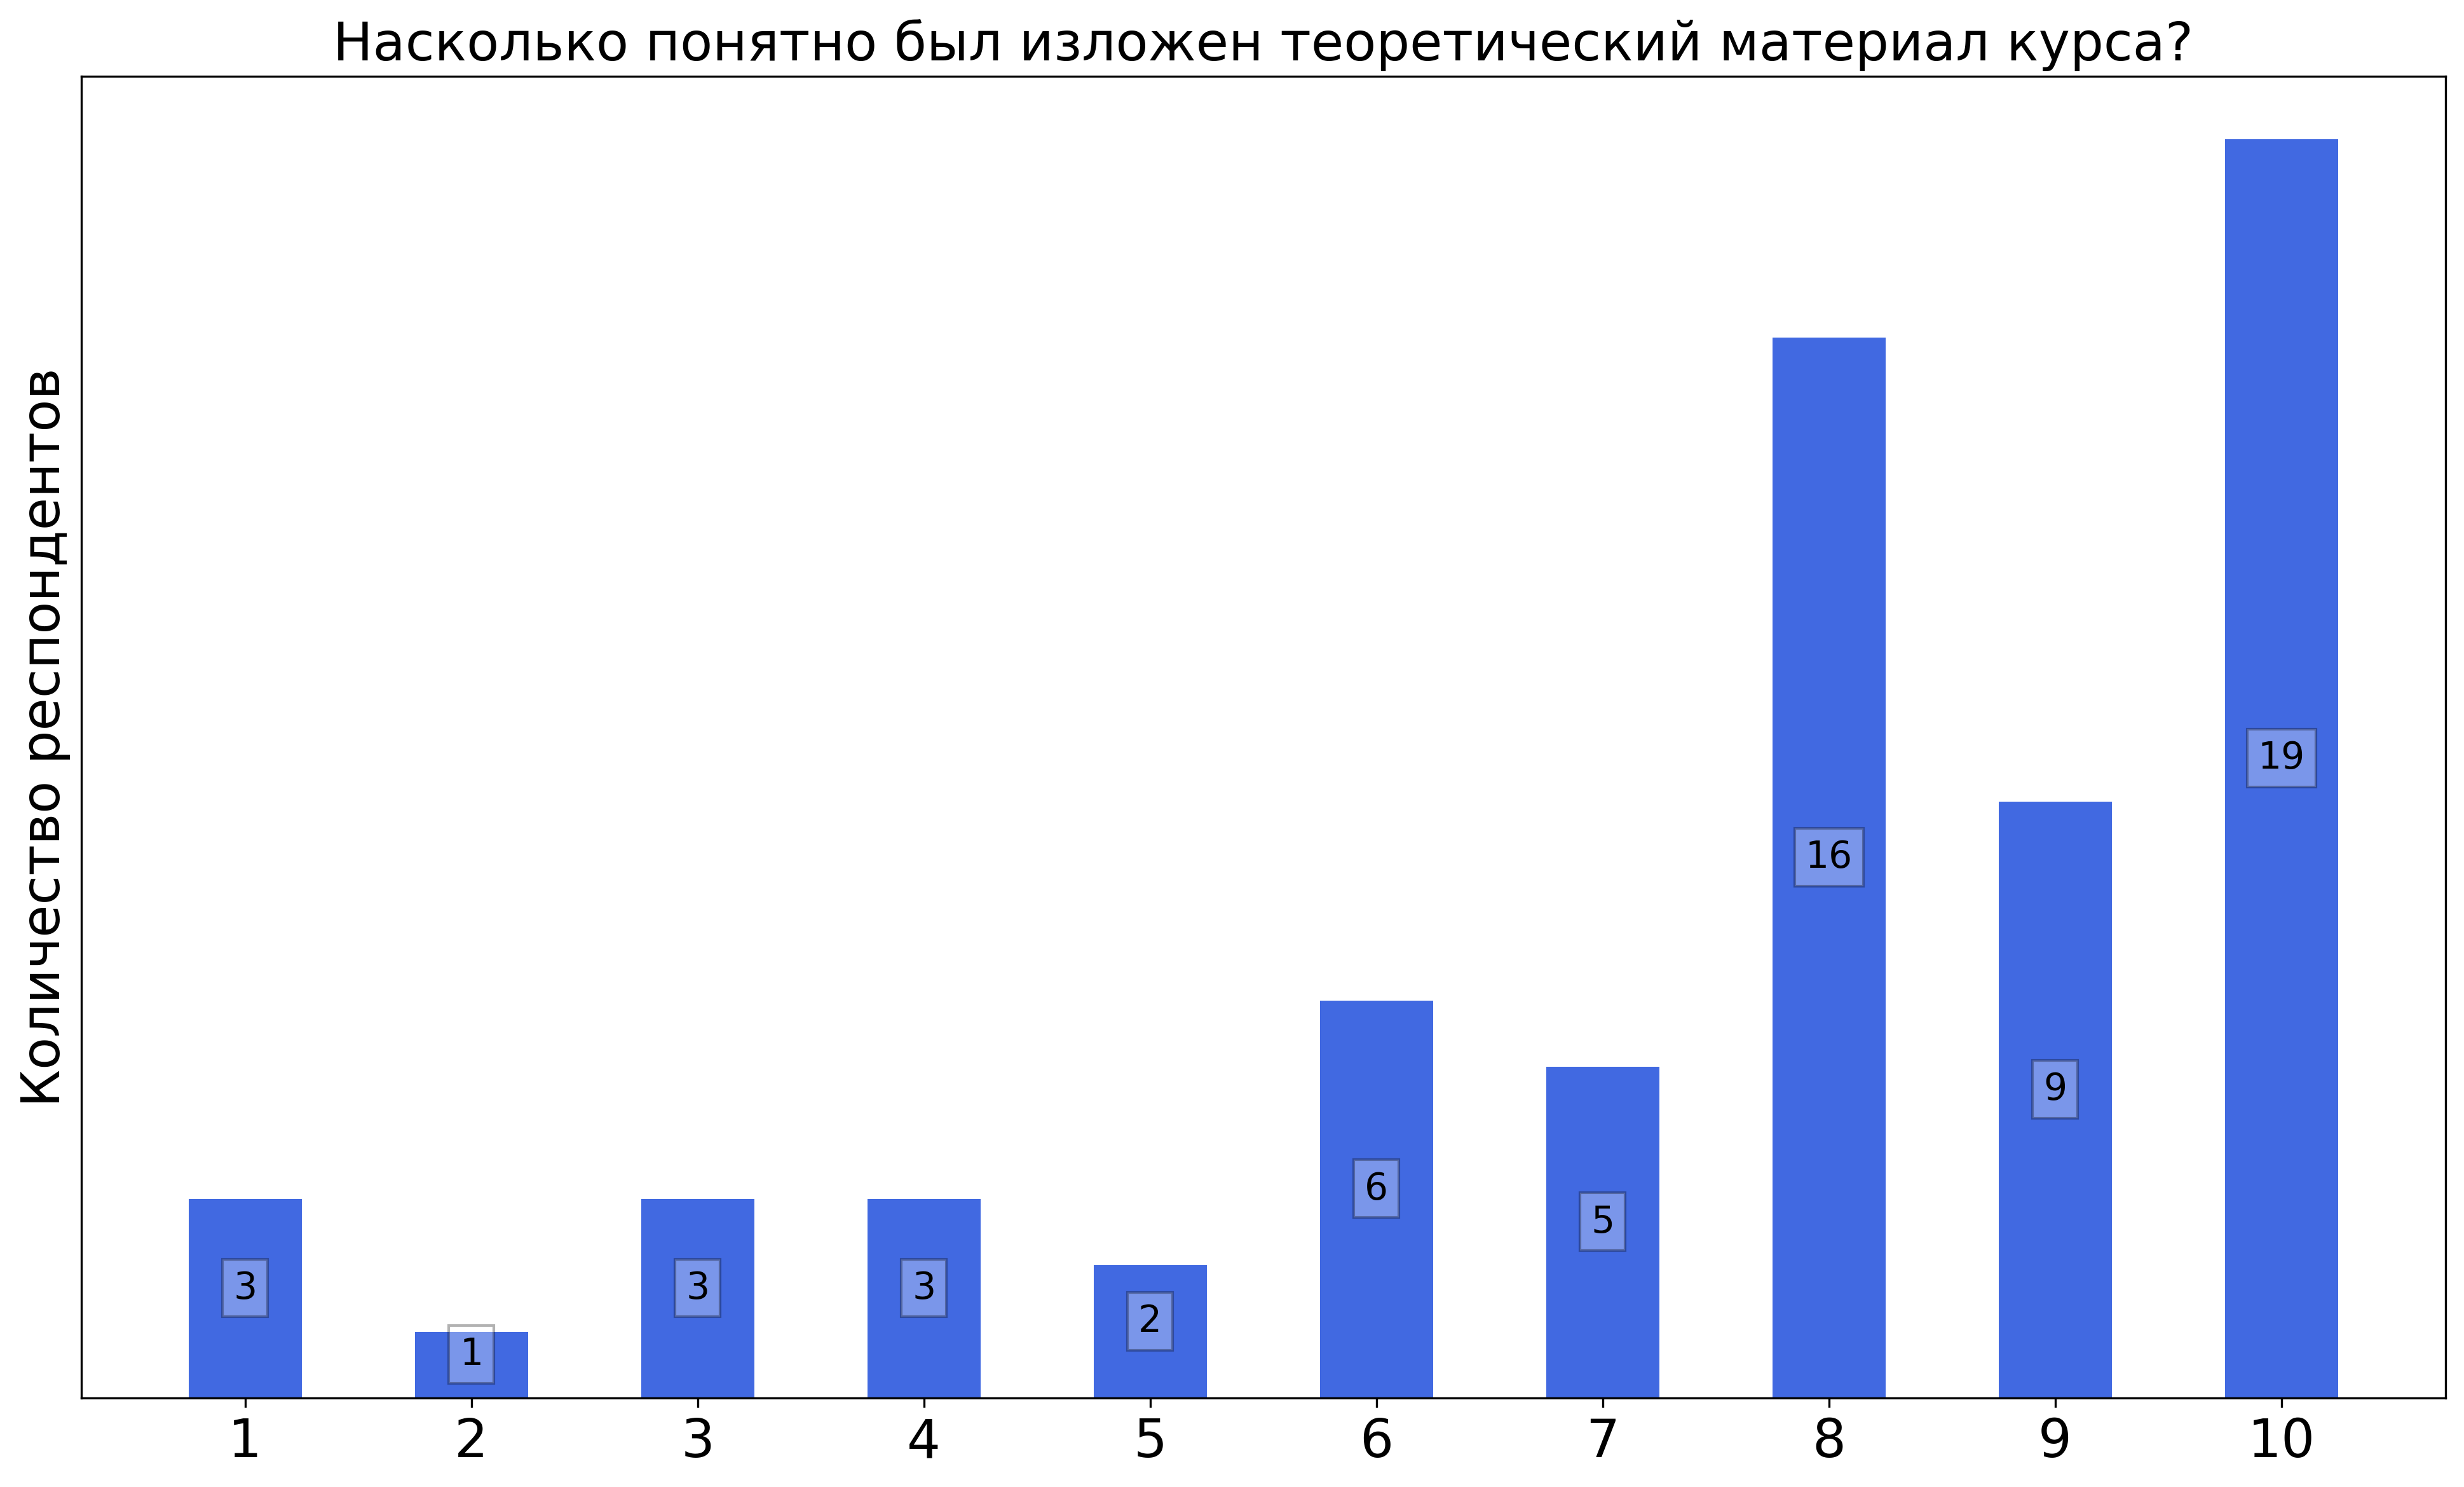
\includegraphics[width=\textwidth]{images/3 course/Компьютерные сети/lecturer-marks-Климанов М.М.-2.png}
			\end{subfigure}
			\begin{subfigure}[b]{0.45\textwidth}
				\centering
				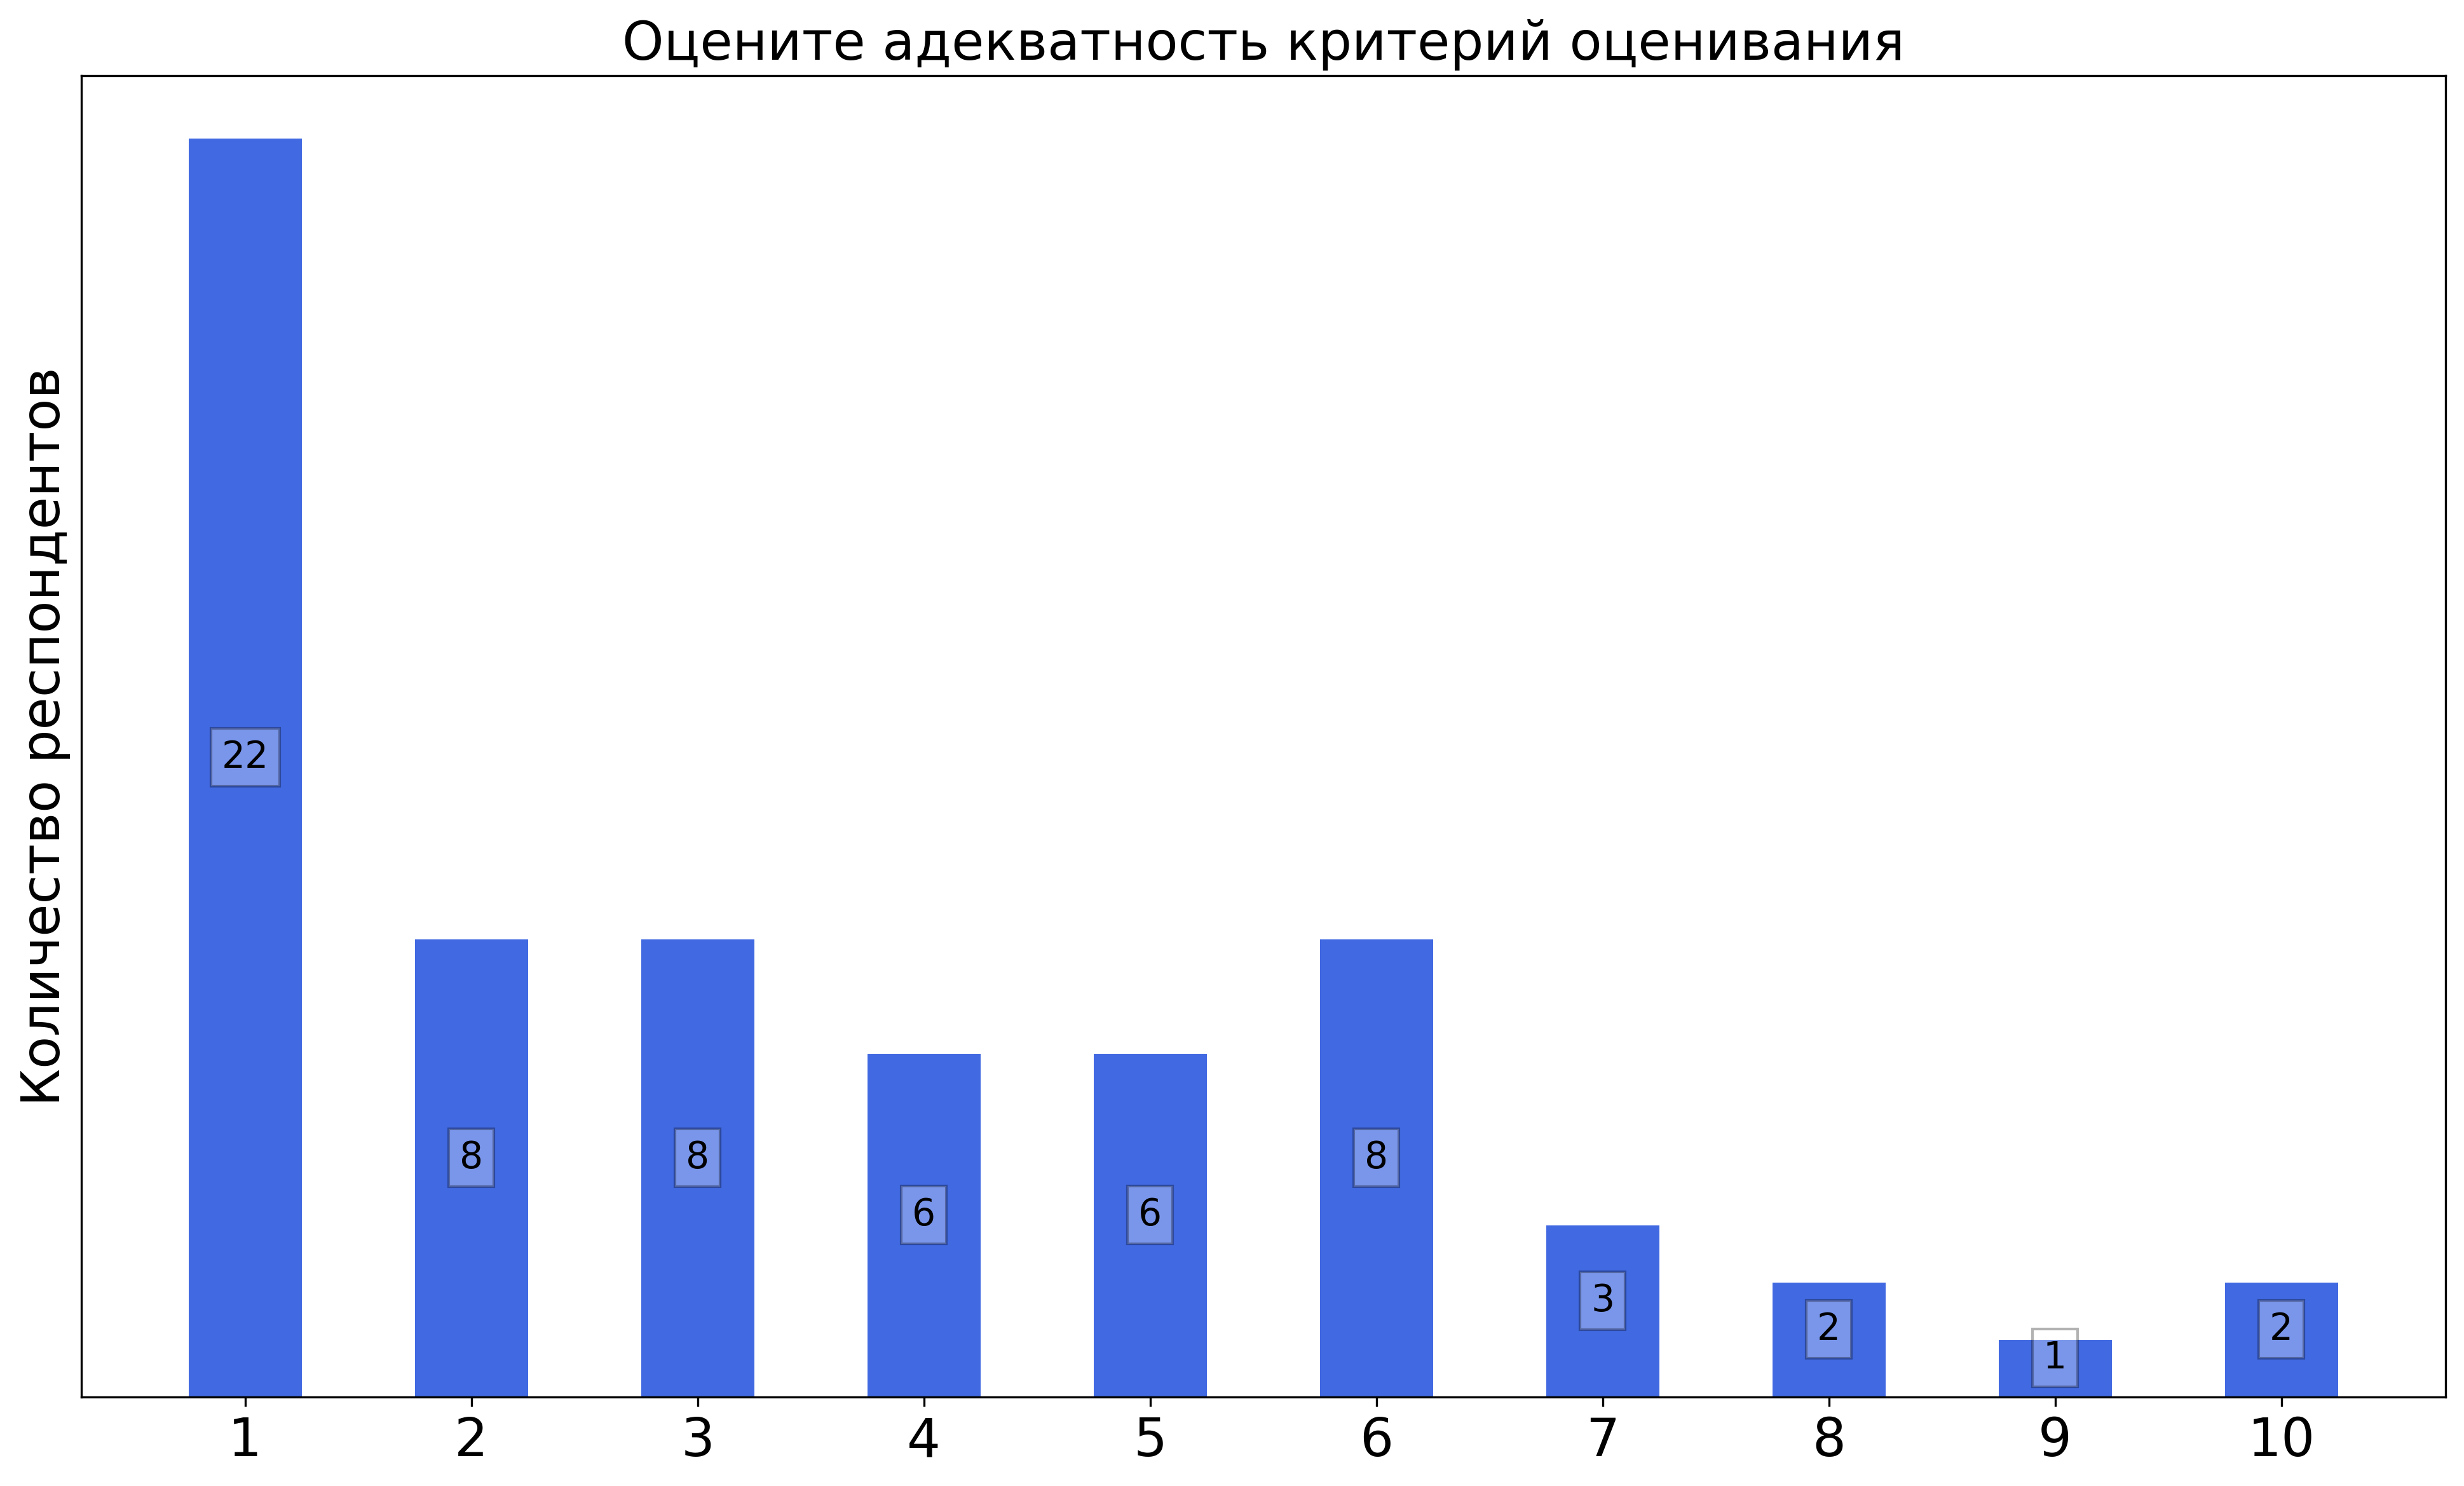
\includegraphics[width=\textwidth]{images/3 course/Компьютерные сети/lecturer-marks-Климанов М.М.-3.png}
			\end{subfigure}
			\caption{Оценки респондентов о качестве преподавания лекций по курсу <<Компьютерные сети>>}
		\end{figure}

		\textbf{Комментарии студентов о лекциях\protect\footnote{сохранены оригинальные орфография и пунктуация}}
            \begin{commentbox} 
                Я думаю, говорить о недостатках не имеет смысла: все и так о них знают. Лектор строгий, жёсткий, а местами и жестокий. Курс в жизни будет очень полезен, читается достаточно хорошо, поэтому, в целом, я доволен 
            \end{commentbox} 
        
            \begin{commentbox} 
                Один из лучших курсов, и один из лучших лекторов на физтехе. При этом совершенно непонятно, зачем вводить несправедливую систему оценивания, а самому лектору так относиться к студентам. Мне кажется, обидеться на студентов, которые не хотели писать тесты через 40 минут после конца последней пары, наказать весь курс чрезмерно сложным тестом, аннулировав при этом предыдущий результат, и попытаться показать пальцем на "виновников" - это детское поведение, а не просто непрофессионализм. 

                Я был на всех лекциях, хорошо написал все тесты, кроме "штрафного", за первую контрольную получил один из лучших среди курса результат.  Но на второй контрольной получил сложный вариант, за него 1,3 балла, которые даже не смог апеллировать, так как уже уехал домой.  Итог - хор(5), за одним исключением худшая оценка за все время обучения. Зачем Максим Михайлович намеренно потрит отношение к себе и телекому, непонятно большинству студентов. 
            \end{commentbox} 
        
            \begin{commentbox} 
                Лектор очень доступно преподносит материал. Лекции интересные. К сожалению, некоторые лекции начинались с опозданием, иногда на 30-40 минут. 
            \end{commentbox} 
        
            \begin{commentbox} 
                Курс шикарен. Лектор показал себя не с лучшей стороны. На обе кр опоздал на 2 часа. Систематически заканчивал лекции позже нужного. Выкинул номер после жалобы на него 
            \end{commentbox} 
        
            \begin{commentbox} 
                Ужасное отношение к студентам, полное отсутствие уважения к людям. 
            \end{commentbox} 
        
            \begin{commentbox} 
                Максим Михайлович отлично разбирается в своем предмете и умеет его объяснять. Это его огромный плюс. Благодаря нему разобрался в основах современных (и не только) компьютерных сетей. Но есть и минус: опоздания на две контрольные. 
            \end{commentbox} 
        
            \begin{commentbox} 
                Весь курс в страхе, специально введён повышающий коэффициент - кажется что-то не так. Лектор готов отвечать на любые вопросы и хочет, чтобы его предмет усвоили - это хорошо. Есть общий чат, удобно. Но задержка лекций, опоздание на них и на контрольные портят всё впечатление о курсе. К тому же, лектор оказался обидчивым. Для освоения есть материалы и ботать теорию в какой-то момент было даже прикольно 
            \end{commentbox} 
        
            \begin{commentbox} 
                Лекции сами по себе очень полезные и приятные. Но когда методы выставления отметок – это просто издевательство над студентами. Летучки, которые могут произойти на любой лекции по любым прошедшим темам еще можно понять и простить, но проведение контрольных и финальное выставление отметок – точно нет. Сначала лектор ставит время контрольной на 18.35,и только через полтора часа, когда у всех уже разболелась голова от нахождения в душной аудитории и волнения, приходит ее проводить. Также отмечу излишнюю строгость при ее проведении: кто хочет, все равно найдет способ списать, а вот простых студентов это только пугает.  

                Если бы этот курс закрывался на хор 7 или отл без каких-то невероятных усилий, то даже такую нервотрепку можно было бы простить. Однако, даже при том, что предмет занимает очень много времени(сравнимо в лабораторными по физике, скорее всего даже больше), он абсолютно не окупается в отметке: в среднем можно рассчитывать на 4-6.
        
                Резюмируя, складывается такое ощущение, что весь курс построен для издевательства над студентами. 
            \end{commentbox} 
        
            \begin{commentbox} 
                Неадекватные критерии оценивания. Ненормально, когда половина потока получают уд, а вторая половина хор. Задержание лекций на 1-1,5 часа. Опоздания на контрольные.  
            \end{commentbox} 
        
            \begin{commentbox} 
                Климанов ужасный человек, сколько нервов он сгубил. Его постоянные опоздания на КР... Не очень понятно, зачем этот человек даёт кр на внимательность и мы после 5 пар сидим в аудитории ждём его 1,5 часа. И когда он наконец приходит мы уставшие пишем его контрольную на внимательность(он сам называл так несколько заданий при разборе). И удивительно, но люди уже теряют возможность внимательно отвечать на вопросы. Отсюда и ужасная статистика оценок за кр. Как лектор к нему вопросов нет, рассказывает интересно, медленно и с примерами. Все понятно. 
            \end{commentbox} 
        
            \begin{commentbox} 
                На вопросы отвечает порой агресивно - нет желания лишний раз что-то у него спрашивать. Тем более, что его ответы иногда могут сильно затянуть лекцию, а на оффициальное время окончание пары лектору глубоко безразлично. Но отвечает точно. понятно и предмет точно знает отлично.

                Отличные лекции (действительно харизматичный лектор), прекрасная методичка, но расстраивает необходимость абсолютной посещаемости лекций, так как каждый год курс меняется и именно изменившиеся детали Климанов использует в тесте (хотя они могли прозвучать всего раз в его лекции и еще 1 раз в методичке). 

                Лучшее изложение не знаю где искать, да и не хочется как будто (возможно есть более глубокие книги, но не уверен, что они лучше для понимания и тем более на русском языке).

                Критерии оценивания слишком жесткие, а тесты настраивают человека не на фактическое понимание предмета, а на поиск тонкостей и подвохов. Нормальное распределение у хор 5,6 - это ненормально.

                Я рад, что у меня был этот предмет и что его ведет такой интересный и знающий человек 
            \end{commentbox} 
        
            \begin{commentbox} 
                Предмет сам по себе интересный. Материал объяснялся подробно.

                Не понравилось отношение преподавателя к студентам. Он опаздывал на лекции до одного часа, особенно на контрольные, из-за чего лекция затягивалась до 21 вечера. Я считаю, что такое не допустимо, учитывая тот факт, что учёба должна заканчиваться в 20:00. Причём, хочется отметить тот факт, что преподаватель никак заранее не уведомлял студентов об опоздании в общем телеграмм канале. Не редко лектор читал лекцию сильно выходя за выделенные рамки пары. Лекция могла начаться ровно в 18:35 и завершиться пол девятого - в девять.  
            \end{commentbox} 
        
            \begin{commentbox} 
                Самая главная проблема этого курса: на лекциях нам читают теорию и не учат решать задачи, на лабораторных работах мы изучаем конфигурацию разных устройств, а в контрольных неожиданную дают задачи, с которыми мы никогда не сталкивались, не отрабатывали навык их решения. Даже если ты вызубришь содержание всех лекций наизусть( и поймешь, как все работает), ты все равно не научишься решать задачи, потому что для этого нужен особый навык. Например, на курсе тфкп чтобы научиться считать интегралы с помощью вычетов недостаточно только лекций, у нас для этого существует отдельный семинар, где ты можешь поучиться, прогибаться и наработать навык. На этом курсе такой практики нет.
        
                Кроме того, критерии оценивания максимально странные: за малейшую неточность в ответе вычитается чуть ли не половина баллов, хотя смысл абсолютно правильный.
        
                Лектор опаздывал на контрольные на 1,5-2 часа. Писать контрольные в 9 часов вечера невероятно трудно, тем более после 2 часов ожидания. Кроме того, лектор неоднократно задерживает после лекций и иногда проводит тесты после официального окончания пары. Я считаю такое отношение к студентам недопустимым со стороны преподавателя.
        
                Сам курс кажется не универсальным, его содержание не позволяет получить полное представление о том, как работают современные сети(мы не проходили ни вай фай, ни сотовую связь). Зато мы углублялись в механизмы, которые на данный момент в современных сетях устарели и не используются 
            \end{commentbox} 
        
            \begin{commentbox} 
                Материал излагается инетресно, но есть большие вопросы к критериям оценивания и опозданиям лектора на свои же контрольные на более чем 2 часа. Не понятно как можно оценивать знания студентов по двум 40 минутным контрольным, где большинство времени занимает прочтение самого задания, к тому же большинство из них рассчитаны больше на внимательность, нежели на проверку знаний. Кажется, что если бы на контрольные давалось побольше времени система оценивания казалась бы более адекватной. К тому же такие вопросы как: "Какова тощина жила в оптоволокне?" не должны сильно влиять на оценку студенты так, как вопросы на понимание конкретных технологий. 
            \end{commentbox} 
        
            \begin{commentbox} 
                Климанов странный человек с непонятно огромными требованиями. Материал классный и нужный, но Климанов все наслаждение растер в пух и прах 
            \end{commentbox} 
        
            \begin{commentbox} 
                Почти единственный курс на физтехе, который был интересен. Как лектор Климанов очень хорош. Если бы ещё и не опаздывал и чуть более по-доброму оценки ставил, цены б ему не было 
            \end{commentbox} 
        
            \begin{commentbox} 
                Крайне недовольна лектором. Для меня  абсолютно неадекватно регулярно опаздывать на лекции (от 15 минут), задерживать на паре (30-40 минут, а пара последняя, в 20 должна заканчиваться).

                Помимо этого на обе контрольные преподаватель опоздал более чем на 1,5 ч. Первую кр начали в 20:05, а вторую уже после 21 вечера. Ни предупреждения, ни извинений, только нахальное поведение по отношению к студентам. После жалобы на задержку первой кр лектор обнулил её результаты и назначил новую со словами "вы знаете, кого благодарить".

                Материал лекций содержательный и полезный, курс мог бы быть интересен, если бы не лектор. 
            \end{commentbox} 
        
            \begin{commentbox} 
                Оценка за курс зависит от контрольных, задания на которых нигде и никогда не освещаются. Единственный способ разобраться как их решать - надеяться на решения кр прошлых лет от старшекурсников(о правильности их решений речи не идёт) 
            \end{commentbox} 
        
            \begin{commentbox} 
                Не приятно, когда были задержки на контрольных в размере пол пары, целой пары. Не было четкой разбаловки за активность в семесте. Она появилась постфактум после выставления всех оценок за все активности.
            \end{commentbox} 
        
            \begin{commentbox} 
                Критерии оценивания на контрольных этого лектора ужасны. На апелляции по контрольной выяснилось, что для полного балла за задачу необходимо было отвечать на вопросы, которые в условии заданы не были 
            \end{commentbox} 
        
            \begin{commentbox} 
                Климанов - самый отвратителььный лектор за все три года на физтехе. Полное неуважение к студентам вызывает нежелание даже просто прикасаться к данному предмету. Про ситуации, которые произошли в течение семестра, вы наверняка наслышаны. Больше всего поразило то, что данный ущемленный человек ни то, что не извинился перед аудиторией, а  ещё и обозлился после жалоб в деканат. После выставления итоговых оценок с фамилией Климанов ассоциируются только нецензурные слова)) Лектор в первую очередь должен вызывать уважение у студентов, здесь такого не наблюдалось никогда. Надеюсь, его наконец-то снимут с поста лектора по компьютерным сетям. 
            \end{commentbox} 
        
            \begin{commentbox} 
                Надменный преподаватель, часто опаздывает, задерживает. Весь поток ждал его на 2й контрольной 2 часа, чтобы написать кр за 40 минут. После того как было написано заявление, высказывался в чате насчет этого заявления. На второй контрольной, после 2х часового ожидания, ехидно спрашивал, все ли готовы писать, зная что бедные студенты просто стерпят. 
            \end{commentbox} 
        
            \begin{commentbox} 
                Лектор опоздал на все контрольные больше чем на полчаса. Неадекватные вопросы в тестах и контрольных, которые в большинстве своём направлены на проверку очень частных фактов, а не на понимание основных концепций.  
            \end{commentbox} 
        
            \begin{commentbox} 
                Лектор предъявляет слишком неадекватные требования к студентам. 
        
                Постоянно опаздывает из-за чего задерживает студентов на 2-3 часа в дни контрольных. Включает в контрольные темы, мельком разобранные в курсе. Большинство вопросов там похожи не на общий курс, а на дотошный разбор спецификаций в технической документации, которые невозможно выучить, не работая сетевым инженером несколько лет. 
                
                Не обновляет свои материалы и постоянно растягивает курс, методичка за наш 2024 год, в три раза больше, чем за 2022. 
                
                Помимо этого, его навыки преподавания оставляют желать лучшего, он рассказывает монотонно, абсолютно не слышит обратную связь от аудитории. На апелляциях не принимает другой точки зрения, требует чтобы ответ был такой, какой он хочет услышать, а не  ответ на вопрос задачи. 
            \end{commentbox} 
        
            \begin{commentbox} 
                Сделать на контрольных более структурированные задачи и сделать ее менее жесткой без флешбеков с егэ.  И без рандомных вопросов в тестах 
            \end{commentbox} 
        
            \begin{commentbox} 
                Климанов М. М. хорош как специалист в своей области. Готов отвечать на вопросы студентов во время лекции, сами лекции читает хорошо и в целом понятно. На этом положительные качества преподавателя резко заканчиваются. 
        
                В остальном это человек крайне непунктуальный, злопамятный, и, мягко говоря, совершенно не уважает студентов и их время. Он нарочно задерживал лекции на минут 30-40 после окончания в самый долгий и трудный учебный день (20:00 - время окончания лекции). "Я задержу лекцию, пользуясь тем, что у вас сегодня больше нет пар" - одна из цитат лектора. Многие ребята уходили после звонка, так как нужно сделать множество дел (поботать, подготовиться к следующему дню и тп). Но Климанов устраивал тесты именно после окончания пары, и эти тесты должны были учитываться при выставлении итоговых оценок. 
                Отдельного внимания заслуживают контрольные работы, вносящие основной вклад в итоговую оценку. С учётом того, что пара длится с 18:30 до 20:00, на проведение первой к.р. лектор пришёл примерно в 19:45, а контрольная началась в 20:05. При этом не было с его стороны предупреждений, извинений и пр. Не было также переноса к.р. На вторую к.р. лектор опоздал по причине "сори, пробки", прийдя в аудиторию приблизительно в 20:00, начало к. р. в 20:15 и конец в 21:00. И это, заметим, в разгар зачётной недели.  
            \end{commentbox} 
        
            \begin{commentbox} 
                Климанов один из лучших лекторов на физтехе. Много знает, и, что очень важно, умеет объяснять материал. Отвечает на все вопросы, старается, чтобы все все поняли. Как человек, своеобразный. На лекции в течение семестра не опаздывал, но на кр задержался на час, что подлило масло в огонь, учитывая и без того большой стресс всего потока перед сложной кр. Еще был непонятный инцидент, когда он дал тест после лекции, про который я думаю и так все знают, после чего повел себя Климанов довольно странно и мерзко. Что касается оценивания знаний - спорный вопрос. С одной стороны, любую вещь, которая была произнесена на лекции, студенты по его мнению должны знать наизусть(по типу порта NTP или что такое TDM и т. д.), времени на его кр мало, реально мало, я только успел сделать последнюю задачу, как время закончилось. Из-за этого из 10 баллов получить больше 5-7 почти нереально, хоть это и компенсируется повышающим коэффициентом. С другой стороны, такой подход готовит студентов к будущему, что в жизни может оказаться все гораздо сложнее, ну и сети хотя бы знать немного будем. Для меня как человека с крекера, считаю курс реально полезным и хорошим, и благодарен за это Климанову,  но если вы студент с другой кафедры, то не будет тяжело, как морально так и физически. 
            \end{commentbox} 
        
            \begin{commentbox} 
                По материалу курс довольно интересный, однако все это портит довольно странное отношение лектора к студентам. Лучше это будет видно на нижеизложенных примерах. Так, Климанов предупреждал, что может опаздывать, однако, что интересно, на лекции он почти не опаздывал (5-10 минут 1-2 раза не в счет), но на обе контрольные работы он опоздал примерно на 1,5 часа. Это было весьма неприятно, поскольку по расписанию пара и так начинается поздно (18:30), а так писать работу в 20:00 и позднее довольно тяжело. Был еще один случай: Климанов задержал на лекции на 40 минут после чего провёл тест. Часть людей не осталась до конца (что вполне нормально, ведь пара должна кончаться в 20:00, а не в 20:40), после этого они обратились в деканат от своего имени. Климанов же решил за такое наказать весь поток, аннулировав этот тест (потом был ещё без задержки, но он был гораздо сложней). По итогу могу сказать, что материал предоставляется весьма интересный, лектор охотно отвечает на возникающие вопросы по предмету, однако такое отношение к студентам оставляет весьма неприятные ощущения. 
            \end{commentbox} 
        
            \begin{commentbox} 
                Много информации в лекции не входило, поэтому приходилось читать дополнительно, очень жёсткие требования и система оценивания 
            \end{commentbox} 
        
            \begin{commentbox} 
                Хочется, чтобы методичка была похожа на методичку, потому что сейчас она больше похожа на учебник по компьютерным сетям. Я бы хотел, чтобы методичку и учебники как-то разделили и добавили в методичку побольше практических задач и разборы некоторых контрольных прошлых лет 
            \end{commentbox} 
        
            \begin{commentbox} 
                Очень хороший теоретический курс - лекции понятны и интересны. Оценивание же - ужас ужасный. Задания на контрольных случайны по сложности, при этом одинаковы по весу. Вполне может сложиться такая ситуация, что человек, почти не учивший сети, решил 3 простейших задания на арифметику, получив 3 балла, также человек, готовившийся к контрольной, допустил ошибку в одной из 3х простых задач (исключительно из за того, что в адресе IPv6 в двух вариантах были перепутаны буквы b и d, чтобы студент этого не заметил и ошибся) и решил 2 более сложные задачи, при этом преподавателю просто не понравился один из ответ студента - он спрашивал про другое, что не отражено в формулировке задания - и он также получает 3 балла, хотя готовился. В общем и целом контрольные разделены на 10 задач по баллу каждая, там 3 задачи очевидны, несколько адекватных задач в стиле описать работу протокола или какого-то его улучшения, задача на сопоставление и несколько сложных задач на ситуации в сети, в которых нужно глубоко разобраться, при этом, как будто студенту нечего делать - ему еще самому нужно назначить адреса на устройства, и уже потом описать, что будет происходить. Правильность этого описания решит исключительно преподаватель. Фактор субъективности огромный, в нескольких задачах встречаются вещи, не рассказанные или вскользь упомянутые в лекциях, и не встречающиеся в методичке лектора. Темы этих вопросов обычно абсолютно избыточно глубоки в какой-то небольшой точке, при этом для общего понимания сетей почти не играют роли. Единственная цель этих вопросов, которую я вижу - завалить студента на контрольной. В общем и целом можно утверждать, что человеческое уважение преподавателя к студентам находится глубоко на дне, несмотря на умение излагать материал. Преподаватель дважды на 1.5 часа опоздал на контрольную (на лекции почти не опаздывал), задерживал на лекциях, что в общем нормально, но через 30-40 минут после конца пары он давал тесты, хотя некоторые люди из за своих (вполне законных) планов после пар уходили после 20.00. после жалобы таких студентов, насколько я знаю, была договоренность провести специально для них дополнительный тест с аналогичными по сложности вопросами, вместо этого результаты теста (достаточно хорошие по всему курсу) были аннулированы, и был проведен дополнительный тест с вопросами "на завалить". После разговора о недопустимости опозданий на лектор снова опоздал на 1.5 часа, в саркастичной манере предложив недовольным покинуть аудиторию. В общем, несмотря на изначально положительные впечатления от лекций, лектор из-за своего неуважения к студентам вызывает лишь негативные ассоциации  
            \end{commentbox} 
        
            \begin{commentbox} 
                Лекции читаются хорошо, всё понятно и структурировано. На вопросы аудитории всегда поступает чёткий ответ. На лекциях разбирается теоретический материал, но не решение задач, которые даются на контрольных,  поэтому у студентов и возникают трудности при их  написании. В пример дали только один вариант контрольной прошлого года. Критерии оценивания абсолютно неадекватные. Со всего курса отличную оценку получили только 6 человек из 150 
            \end{commentbox} 
        
            \begin{commentbox} 
                Сами лекции читаются прекрасно, Климанов рассказывает интересно и всегда отвечает на вопросы аудитории. Однако система оценивания по предмету абсолютно неадекватна, ибо оценка формируется по большей части по результатам контрольных, на которых даются задачи, решение которых в принципе в лекциях не разбирается. Сам курс теоретический, а в качестве контроля предполагает решение задач, додуматься до которого зачастую не возможно, не имея опыта. Также несмотря на прекрасное изложение материала лектор отвратительно относился к студентам, регулярно задерживая их на пол часа или 40 минут (т. е. до 20:30-20:40). На контрольные же Климанов и вовсе оба раза явился в 8 вечера, даже не предупредив об этом, тем самым проявив абсолютное неуважение к аудитории. Сам же курс и вовсе не нужен практически никому на ФРКТ, поэтому было бы лучше, если бы он был обязательным только для студентов кафедр, связанных с компьютерными сетями, и факультативным для всех остальных. Систему же оценивания необходимо кардинально менять, переводя контрольные в проверку исключительно теоретических знаний в формате тестов без задач. Также хотелось бы, чтобы лектор не задерживал студентов допоздна и в принципе лучше к ним относился. 
            \end{commentbox} 
        
            \begin{commentbox} 
                Объемные курс, который прям необходимо ботать весь семестр. Очень сложно получить высокую оценку.
        
                В отличие от предыдущих семестров, на лекции Климанов почти не опаздывал. НО опаздал на обе контрольные (на 1.5 и 2 часа соответственно). Кроме того, иногда задерживал после пары. 
            \end{commentbox} 
        
            \begin{commentbox} 
                Курс достаточно прост для понимания, теоретический материал не вызывает сложностей в освоении. Лектор открыт для студентов и готов отвечать на вопросы и пояснять материал. Поведение же лектора по отношению к студентам ужасное, частые опаздывания на более чем полчаса на лекцию (на первую контрольную на лекции лектор явился спустя полтора часа, т.е. после окончания лекции, и контрольная всё равно была проведена). Тесты проводимые на лекциях (тоже иногда после окончания) аннулируются с легкой руки, как будто специально, чтобы снизить итоговые баллы. Все действия лектора по ощущениям направлены на то, чтобы завалить студентов. Контрольные непропорционально сложные относительно преподаваемой теории и оцениваются слишком строго для курса без экзамена (половина курса слетело со стипендии, только у 7\% вышел отл), задачи с контрольной на лекциях не разбираются и материалов для подготовки также недостаточно, что делает получение оценки по курсу рандомным. 
            \end{commentbox} 
        
            \begin{commentbox} 
                О лекторе: не уважает чужое время, обижается на адекватные претензии из-за организации лекций и контрольных, в следствии чего карает сложностью заданий на контрольных и тестах 
            \end{commentbox} 
        
            \begin{commentbox} 
                Отвратительная система выставления оценки за курс всего по двум контрольным работам. Контрольные работы - тот еще отврат, даже если хорошо ориентируешься в курсе - сложно написать больше чем на 3 балла. Задачи с подвохом, требование к идеальному знанию каждого нюанса курса - мерзость. Чтобы получить что-то приемлемое - нужно заучить. Да даже эта великолепная система с повышающим коэффициентом о чем-то да говорит. Очень не понравилось, хоть и в сетях я неплохо разобрался. 
            \end{commentbox} 
        
            \begin{commentbox} 
                Много материалов и на лектор готов много времени уделять студентам, но некоторые моментами с задержками лекций, опозданиями и системой оценивания напрягли 
            \end{commentbox} 
        
            \begin{commentbox} 
                Человек харизматичный но высокомерный. Из лекций ничего не вынес, лучше изучать самому. Система оценивания отвратительна. Опоздал на контрольную на 1.5 часа! 
            \end{commentbox} 
        
            \begin{commentbox} 
                Лектор очень обидчивый! Подает материал интересно, но его отношение к временам конца и начала пары и к нашим мнениям сильно отталкивают. Из-за того, что пару человек пожаловалась, что у нас задержали конец пары почти на час (пара должна была кончиться в 20.00, закончилась в 20.50), лектор обиделся, отменил результаты теста, который он провел в 20.45, когда уже пара человек довольно законно ушли и дал тест, который даже старательные студенты сильно хорошо не написали. 2/10 средний балл за тест. 
            \end{commentbox} 
        
            \begin{commentbox} 
                Лектор абсолютно неадекватно проводит контрольные (пара начиналась в 18:35, первая контрольная началась в 20:05, вторая - в 20:15), полный абсурд. В контрольных было много задач - ловушек, на внимательность, что абсолютно невыносимо, учитывая поздний вечер и задержку начала почти на 1.5 часа. Требуется знать какие-то незначительные детали, типо толщины оптоволоконной жилы или количества бит в поле какого-то заголовка какого-то протокола, что частично превращает в зазубривание. 
            \end{commentbox} 
        
            \begin{commentbox} 
                На лекциях очень много ненужной теории, которая никогда в жизни не пригодится. Например, нужно знать диаметр какого-то провода или сколько битов в определенном поле заголовка. И потом эти вопросы спрашиваются на тестах. Непонятно, для чего это надо знать. Даже если идти работать в сферу сетей/ телекоммуникации, вся эта информация гуглится за пару минут, нет никакого смысла все это помнить.

                Про организацию учебного процесса: Климанов позволил себе опоздать на обе контрольные на 1,5-2 часа, при этом точное время прихода он не говорил, и весь курс был вынужден все это время сидеть ждать его в аудитории. Никаких извинений за опоздания не было. На студентов смотрит сверху вниз, общается максимально пренебрежительно. Когда группа студентов пошла жаловаться в деканат с просьбой дать им написать тест, с которого они ушли, потому что Климанов задержал окончание лекции на 40 минут, Климанов вместо того, чтобы выполнить распоряжение деканата и провести отдельный тест для этих студентов, обнулил всему потоку этот тест и написал в общий чат, что "вы знаете, кого за это благодарить". На мой взгляд, это очень непрофессиональное поведение. Вместо того, чтобы признать свою ошибку, Климанов обвинил студентов в том, что они пошли жаловаться, и попытался стравить студентов между собой. И после этого он намеренно дал всему потоку очень сложный тест, который студенты написали намного хуже, чем предыдущие тесты.

                Я считаю, что такое отношение к студентам со стороны преподавателя недопустимо. 
            \end{commentbox} 
        
            \begin{commentbox} 
                Лектор - крайне неприятный в общении человек, хоть и объясняет вроде интересно, с готовностью отвечает на вопросы.  К студентам относится бех алейшего уважения и понимания, задерживает лекции и опаздал на обе контрольные на 1.5 часа
                Система выставления оценок - полный рандом, совершенно не справедливо
                Мне, как человеку, никогда не интересовавшемуся сетями, было трудно, неинтересно и неприятно изучать курс, хотя я старалась и методичку читала. 
            \end{commentbox} 
        
            \begin{commentbox} 
                1. Несбалансированный, чрезмерно глубокий и при этом в большинстве своём пустой курс. Ртшников на 3м курсе можно условно разделить на 2 типа: ребята, которые хотят плотно развиваться именно в сфере телекома, и остальных, кому телеком в какой-то мере все нужен, однако скорее как инструмент для развития навыком в другой области. Первых у нас от силы процентов 10. (Кафедра неткрекера = 14 человек ~150 на потоке). Естественная ступень профессионального развития сетевого инженера - аккредитация с помощью экзамена Cisco (Климанов не раз говорил про него). Для остальных сдача конкретно этого экзамена не представляет никакого интереса, а вот что представляет - так это понимание общего устройства сети (преимущественно верхней части, начиная с транспортного уровня TCP/UDP) и некоторые прикладные знания по взаимодействию с протоколами верхних уровней (В особенности они интересуют людей, деятельность которых связана с программированием, а таких многократно больше, чем тех же сетивиков). Что мы наблюдаем: курс Климанова не закрывает потребности ни тех, ни других. Полное его усвоение всё равно не подготовит студента к сдаче cisco-экзамена, и в то же время курс абсолютно не покрывает пробелы студентов, которые хотят иметь общее понимание устройства сети. Т.е. выходит, в курске нет ни глубины, ни ширины. Просто колоссальное количество лекционного времени уходит на какие-то очень узкие, не имеющие для большинства студентов никакого прикладного значения вещи: физический уровень, (вплоть до полировки кабелей), кучу разных версий одних и тех же протоколов (начиная от самых старых) и т.д. В один из дней, подробнейшим образом обсуждая протокол STP, мы задержались на лекции более чем полчаса, только чтобы в конце узнать, что сейчас он неактуален и от него стараются отказываться везде, где только можно - весьма разочаровывает. 
        
                2. Отдельная тема - контрольные Климанова. Обычно все курсы на физтехе состоят из лекций и семинаров. На лекциях - проходим теорию, на семинарах - решаем задачи и пишем контрольную по схожим темам. На курсе сетей же семинаров нет, то есть набить руку и научиться решать задачи, предлагаемые на контрольных, попросту негде. При этом формат контрольной, а именно 10 текстовых задач на 40 минут, будто бы предполагает, что у студентов набита рука на подобные задачи. Да, как правило, на контрольных бывает 2-3 тривиальные задачи, но они вообще слабо относятся к сетям и не отражают никаких общих знаний. В итоге, на мой взгляд, контрольная полностью оторвана от курса, нет никакого внятного механизма подготовки к ней, подавляющее большинство решает только те самые тривиальные задачи, которые стоят столько же, сколько сложные. Получается, что прилежный и ботающий студент получает на кр в среднем не сильно больше баллов, чем раздолб. Контрольная практически полностью теряет смысл. 
            \end{commentbox}


        \subsubsection{Прочие комментарии и предложения по улучшению курса}
            См. соответствующую секцию в отзывах о курсе <<Лаборатория инфокоммуникационных технологий>>.
